\documentclass[12pt,a4paper]{article}

% ── Packages ─────────────────────────────────────────────────────────────────
\usepackage[margin=2.5cm]{geometry}
\usepackage{amsmath, amssymb, amsfonts, amsthm}
\usepackage{graphicx}

\newtheorem{theorem}{Theorem}
\newtheorem{corollary}[theorem]{Corollary}
\usepackage{booktabs}
\usepackage{hyperref}
\usepackage{xcolor}
\usepackage{caption}
\usepackage{subcaption}
\usepackage{microtype}

\hypersetup{
  colorlinks=true,
  linkcolor=blue!60!black,
  citecolor=green!50!black,
  urlcolor=blue!70!black,
}

% ── Custom commands ───────────────────────────────────────────────────────────
\newcommand{\eps}{\varepsilon}
\newcommand{\baseline}{\beta}  % baseline activation = delta/(delta+gamma)
\newcommand{\thr}{\tau}        % threshold

\title{\textbf{Analysis of the Recovery Rate and Separation Quality Dip\\
at Narrow Generation Angles in the Hit-Competition Study}\\[0.5em]
{\large \texttt{hit\_competition\_study.ipynb} — Toy Characterisation Series}}

\author{G.\ Scriven\\[0.3em]
Quantum Track Reconstruction Study\\
LHCb VELO Toy Model}

\date{April 2026}

% ─────────────────────────────────────────────────────────────────────────────
\begin{document}
\maketitle
\tableofcontents

\newpage

% =============================================================================
\section*{Notation and Symbols}
\label{sec:notation}
\addcontentsline{toc}{section}{Notation and Symbols}

The following tables collect every symbol used in this report, grouped by
category.

\subsubsection*{Detector Geometry}
\begin{tabular}{@{}lp{10.5cm}@{}}
  \toprule
  Symbol & Definition \\
  \midrule
  $M$ & Number of detector modules (= 5) \\
  $\Delta z$ & Longitudinal spacing between consecutive modules (= 33\,mm) \\
  $z_k$ & $z$-position of module $k$ ($z_1{=}100,\;z_2{=}133,\;z_3{=}166,\;z_4{=}199,\;z_5{=}232$\,mm) \\
  $z_0$ & $z$-position of the primary vertex (= 50\,mm) \\
  $L_{x,y}$ & Detector half-size in the transverse plane (= 50\,mm) \\
  \bottomrule
\end{tabular}

\bigskip
\subsubsection*{Physics and Generation Parameters}
\begin{tabular}{@{}lp{10.5cm}@{}}
  \toprule
  Symbol & Definition \\
  \midrule
  $n$ & Number of tracks per event \\
  $\phi_\text{max}$, $\theta_\text{max}$ & Half-angle of the generation cone in $\phi$ and $\theta$ \\
  $A_\text{cone}$ & Angular area of the generation cone $= (2\phi_\text{max})^2$ \\
  $N_\text{rep}$ & Number of independent repeat events per density point \\
  $\sigma_\text{res}$ & Hit position resolution (= 0\,mm in this study) \\
  $\sigma_\text{scatt}$ & Multiple-scattering angular width (= $10^{-4}$\,rad) \\
  $k$ & Acceptance scale factor for the angular tolerance (= 3.0) \\
  $\theta_\text{min}$ & Minimum angular offset (= $1.5\times10^{-5}$\,rad) \\
  $\theta_r$ & Angular resolution term $= \arctan(k\,\sigma_\text{res}/\Delta z)$ \\
  \bottomrule
\end{tabular}

\bigskip
\subsubsection*{Hamiltonian Model Parameters}
\begin{tabular}{@{}lp{10.5cm}@{}}
  \toprule
  Symbol & Definition \\
  \midrule
  $\eps$ & Angular acceptance tolerance for segment coupling (= 0.425\,mrad); defined by Eq.~\eqref{eq:epsilon} \\
  $\gamma$ & Self-interaction (diagonal penalty) weight (= 1.5) \\
  $\delta$ & Bias term (= 1.0) \\
  $\baseline$ & Baseline activation $= \delta/(\delta+\gamma)$ (= 0.400) \\
  $\thr$ & Decision threshold $= (1+\baseline)/2$ (= 0.700) \\
  \bottomrule
\end{tabular}

\bigskip
\subsubsection*{Segment and Matrix Quantities}
\begin{tabular}{@{}lp{10.5cm}@{}}
  \toprule
  Symbol & Definition \\
  \midrule
  $N_\text{seg}$ & Total number of candidate segments $= (M-1)\,n^2$ \\
  $\mathbf{A}$ & Hamiltonian system matrix (stored form: positive diagonal, negative off-diagonal) \\
  $A_{ij}$ & Entry of the system matrix at row $i$, column $j$ \\
  $\mathbf{x}$ & Activation vector; solution of $\mathbf{A}\mathbf{x} = \mathbf{b}$ \\
  $x_i$ & Activation value for segment $i$ \\
  $\mathbf{b}$ & Bias vector; $b_i = \delta$ for all segments \\
  $\theta_{ij}$ & Pairwise angle between the direction vectors of segments $i$ and $j$ \\
  $\langle\text{occ}\rangle$ & Mean hit occupancy $= 2\,N_\text{seg}/(M\,n)$ \\
  \bottomrule
\end{tabular}

\bigskip
\subsubsection*{Cross-Segment and Degeneracy Quantities}
\begin{tabular}{@{}lp{10.5cm}@{}}
  \toprule
  Symbol & Definition \\
  \midrule
  $f_\text{amp}$ & Cross-angle amplification factor $= (z_k - z_0)/\Delta z$; maximum value $\approx 3.5$ at module $k{=}3$ \\
  $\theta_\text{cross}^{(k)}$ & Kink angle at module $k$ between a true segment and a cross-segment; Eq.~\eqref{eq:cross_angle} \\
  $\Delta\phi_\text{eff}$ & Effective angular separation between two tracks in 2-D angular space; Eq.~\eqref{eq:tolerance} \\
  $\phi_\text{crit}$ & Critical separation threshold $= \eps / f_\text{amp}^{\max} \approx 0.12$\,mrad \\
  $p_\text{pair}$ & Probability that a specific pair of tracks is near-coincident; Eq.~\eqref{eq:ppair} \\
  $N_\text{degen}$ & Expected number of near-coincident pairs per event; Eq.~\eqref{eq:ndegen} \\
  \bottomrule
\end{tabular}

\bigskip
\subsubsection*{Linear Algebra and Spectral Analysis}
\begin{tabular}{@{}lp{10.5cm}@{}}
  \toprule
  Symbol & Definition \\
  \midrule
  $\kappa(A)$, $\kappa$ & Condition number of matrix $\mathbf{A}$ \\
  $\kappa_2(A)$ & 2-norm condition number $= |\lambda_\text{max}|/|\lambda_\text{min}|$ (symmetric matrices) \\
  $\lambda_i$ & $i$-th eigenvalue of $\mathbf{A}$ \\
  $\lambda_\text{max}$, $\lambda_\text{min}$ & Largest and smallest eigenvalues of $\mathbf{A}$ \\
  $\sigma_i$ & $i$-th singular value of $\mathbf{A}$ (from the SVD $A = U\Sigma V^T$) \\
  $\sigma_1$, $\sigma_n$ & Largest and smallest singular values; $\kappa = \sigma_1/\sigma_n$ \\
  $U$, $\Sigma$, $V^T$ & Matrices of the singular value decomposition \\
  $D_i$ & Gershgorin disc for row $i$: $\{z \in \mathbb{C} : |z - A_{ii}| \leq R_i\}$ \\
  $R_i$ & Gershgorin radius $= \sum_{j\neq i}|A_{ij}|$ \\
  $\rho_i$ & Gershgorin ratio $= R_i / |A_{ii}|$; diagonal dominance violated when $\rho_i > 1$ \\
  \bottomrule
\end{tabular}

\bigskip
\subsubsection*{Performance and Statistical Quantities}
\begin{tabular}{@{}lp{10.5cm}@{}}
  \toprule
  Symbol & Definition \\
  \midrule
  $\langle x_\text{true}\rangle$ & Mean activation over all true segments \\
  $\langle x_\text{false}\rangle$ & Mean activation over all false segments \\
  $\sigma_{x_\text{true}}$, $\sigma_{x_\text{false}}$ & Standard deviation of true / false segment activations \\
  $d$ & Cohen's $d$ (pooled separation quality); Eq.~\eqref{eq:cohend} \\
  Recovery (\%) & Fraction of true segments with $x_i \geq \thr$ \\
  $\langle\sum x_\text{false}\rangle$ & Mean summed activation of false competitors per hit (Step~3) \\
  $N_\text{competitors}$ & Number of false-segment competitors per hit (Step~3) \\
  \bottomrule
\end{tabular}

\newpage

% =============================================================================
\section{Executive Summary}
\label{sec:summary}

The \texttt{hit\_competition\_study.ipynb} notebook evaluates the
\emph{classical} Hamiltonian track-reconstruction method across a range of
track densities and angular generation settings.
Step~2 of that study (Activation Spectrum) reveals a striking \emph{localised
dip} in the true-segment recovery rate and separation quality when the particle
generation cone is set to $\phi_{\max} = \theta_{\max} = \pm0.04$\,rad at a
track multiplicity of 75 tracks per event:

\begin{itemize}
  \item Recovery rate drops from $\approx100\%$ (all other densities) to
        $82.7\%$.
  \item True\,/\,false separation quality collapses from the nominal
        ${\approx}5.4\,\sigma$ to $0.06\,\sigma$ — effectively \emph{no
        separation}.
  \item True-segment activation values span the pathological range
        $[-75.1,\;+154.0]$, far outside the physical interval $[0,1]$.
\end{itemize}

\noindent The root cause is a \textbf{near-coincident track degeneracy}: when
two randomly generated tracks land within the Hamiltonian's angular-acceptance
window ($\sim\!0.12$\,mrad in 2-D angular space), the normally block-diagonal
linear system acquires spurious off-diagonal couplings.
In the most severe cases the system matrix becomes \textbf{indefinite}
(acquires negative eigenvalues), causing the
Conjugate Gradient (CG) solver to diverge catastrophically.
Contrary to earlier reports, the system is \emph{not} truly ill-conditioned
(the SVD-based condition number remains moderate at $|\kappa| \approx 7\text{--}30$);
the widely quoted ``exploding $\kappa \sim 10^{15}$'' was a measurement artefact
from applying a positive-definite formula to an indefinite matrix.
\textbf{The matrix indefiniteness is a potential concern}
that warrants further investigation: it means the CG solver is being applied
to a system that violates its fundamental preconditions.
The dip is confined to a single density point because it arises from a rare
stochastic event in a small ($N_\text{rep}=5$) sample, amplified by the
$25\times$ higher track density in angular space compared with the $\pm0.2$\,rad
setting.

% =============================================================================
\section{Study Configuration}
\label{sec:config}

\subsection{Geometry and Physics Parameters}

The study uses a 5-module planar detector toy model with the parameters listed
in Table~\ref{tab:params}.

\begin{table}[h!]
  \centering
  \caption{Fixed physical parameters used in the hit-competition study.}
  \label{tab:params}
  \begin{tabular}{llr}
    \toprule
    Parameter & Symbol & Value \\
    \midrule
    Module spacing & $\Delta z$ & $33.0$\,mm \\
    Detector half-size & $L_{x,y}$ & $50.0$\,mm \\
    Number of modules & $M$ & 5 \\
    Position resolution & $\sigma_\text{res}$ & $0.0$\,mm (perfect) \\
    Multiple-scattering width & $\sigma_\text{scatt}$ & $1\times10^{-4}$\,rad \\
    Acceptance scale & $k$ & 3.0 \\
    Angular tolerance (epsilon) & $\eps$ & $0.425$\,mrad \\
    Self-interaction (diagonal penalty) & $\gamma$ & 1.5 \\
    Bias term & $\delta$ & 1.0 \\
    Baseline activation & $\baseline = \delta/(\delta+\gamma)$ & 0.400 \\
    Decision threshold & $\thr = (1+\baseline)/2$ & 0.700 \\
    \bottomrule
  \end{tabular}
\end{table}

\noindent The angular tolerance is set by
\begin{equation}
  \eps = \sqrt{2\,(k\,\sigma_\text{scatt})^2 + 12\,\theta_r^2 + 2\,\theta_\text{min}^2},
  \label{eq:epsilon}
\end{equation}
where $\theta_r = \arctan(k\,\sigma_\text{res}/\Delta z) = 0$ (no resolution
error) and $\theta_\text{min}=1.5\times10^{-5}$\,rad.
Numerically, $\eps = \sqrt{2\,(3\times10^{-4})^2 + 2\,(1.5\times10^{-5})^2}
\approx 4.248\times10^{-4}$\,rad $= 0.425$\,mrad.

\subsection{Scan Settings}
\label{sec:scan}

Three generation angle settings are compared (Table~\ref{tab:scan}), crossing
eight track-density points with $N_\text{rep}=5$ events each.

\begin{table}[h!]
  \centering
  \caption{Generation angle settings and their implications.}
  \label{tab:scan}
  \begin{tabular}{lrrr}
    \toprule
    Label & $\phi_\text{max}$ (rad) & Cone area ($\pi\phi^2$, mrad$^2$) &
    Track density at $n=75$ (tracks\,mrad\textsuperscript{$-2$}) \\
    \midrule
    $\pm0.2$ & $0.200$ & $126{,}000$ & $0.60$ \\
    $\pm0.1$ & $0.100$ & $31{,}400$ & $2.39$ \\
    $\pm0.04$ & $0.040$ & $5{,}030$ & $14{,}900$ \\
    \bottomrule
  \end{tabular}
\end{table}

\noindent Note that the $\pm0.04$\,rad setting packs tracks
\textbf{25$\times$ more densely} in angular space than $\pm0.2$\,rad
at equal track multiplicity.

% =============================================================================
\section{The Hamiltonian Linear System}
\label{sec:hamiltonian}

\subsection{Segment Construction}
\label{sec:segments}

For a 5-module detector with $n$ tracks (one hit per module per track), the
Hamiltonian constructs segments for \emph{all} hit pairs across consecutive
module pairs without any angular pre-filtering.
The total number of constructed segments is therefore
\begin{equation}
  N_\text{seg} = (M-1)\,n^2 = 4\,n^2.
  \label{eq:nseg}
\end{equation}
At $n=75$ tracks: $N_\text{seg} = 22{,}500$ total, of which $4n = 300$ are
\emph{true} segments (one per track per module pair) and 22{,}200 are
\emph{false} candidates.

Each internal hit at module $k$ appears in $n$ incoming segments
(from module $k-1$ to $k$) and $n$ outgoing segments
(from module $k$ to $k+1$), giving a mean hit occupancy:
\begin{equation}
  \langle\text{occ}\rangle = \frac{2\,N_\text{seg}}{M\,n}
  = \frac{8n}{5}.
  \label{eq:occ}
\end{equation}
Crucially, this occupancy is \emph{independent of generation angle} — it is
determined entirely by track multiplicity and geometry.

\subsection{Matrix Structure}
\label{sec:matrix}

The linear system $\mathbf{A}\,\mathbf{x} = \mathbf{b}$ has:
\begin{itemize}
  \item \textbf{Diagonal}: $A_{ii} = \delta + \gamma = 2.5$ for every segment $i$.
  \item \textbf{Off-diagonal}: $A_{ij} = -1$ (coupling) if segments $i$ and $j$
    share a common \emph{middle} hit across three consecutive modules
    \emph{and} the pairwise angle between their direction vectors satisfies
    $\theta_{ij} < \eps$.
  \item \textbf{Bias}: $b_i = \delta = 1$ for all segments.
\end{itemize}
The system is solved with \texttt{scipy.sparse.linalg.cg} (Conjugate Gradient,
relative tolerance $10^{-5}$).

\subsection{Idealised Analytic Solution}
\label{sec:analytic}

\paragraph{False segments (uncoupled):}
Because cross-segment angles greatly exceed $\eps$ for non-coincident tracks,
false segments have \emph{no} off-diagonal couplings to other segments.
Their equations decouple:
\begin{equation}
  (\delta + \gamma)\,x_i = \delta \quad \Rightarrow \quad
  x_i = \frac{\delta}{\delta+\gamma} = \baseline = 0.4.
  \label{eq:false_sol}
\end{equation}

\paragraph{True segments (chain-coupled):}
For a single track spanning 5 modules, the 4 true segments form a
tri-diagonal chain:
\begin{equation}
  \begin{pmatrix}
    2.5 & -1  & 0   & 0 \\
    -1  & 2.5 & -1  & 0 \\
    0   & -1  & 2.5 & -1 \\
    0   & 0   & -1  & 2.5
  \end{pmatrix}
  \begin{pmatrix} x_0 \\ x_1 \\ x_2 \\ x_3 \end{pmatrix}
  =
  \begin{pmatrix} 1 \\ 1 \\ 1 \\ 1 \end{pmatrix}.
  \label{eq:true_chain}
\end{equation}
The solution (by symmetry $x_0=x_3$, $x_1=x_2$) gives
$x_0 = 10/11 \approx 0.909$ and $x_1 = 14/11 \approx 1.273$.
All four values exceed the threshold $\thr=0.7$, giving $100\%$ true-segment
recovery per track.

These analytic predictions match the empirical Step~2 results for all
well-behaved events: true mean activation $\approx 1.091$ and false mean
$= 0.400$ exactly.

% =============================================================================
\section{Observed Anomaly at $\pm0.04$\,rad, 75 Tracks}
\label{sec:anomaly}

Table~\ref{tab:step2} and Figure~\ref{fig:step2_summary} summarise the Step~2
activation metrics from the run on 25 February 2026.

\begin{table}[h!]
  \centering
  \caption{Step~2 activation metrics for $\pm0.04$\,rad generation angle.
           Bold row marks the anomalous density point.}
  \label{tab:step2}
  \begin{tabular}{rrrrrr}
    \toprule
    Tracks & $\langle x_\text{true}\rangle$ & $\sigma_{x_\text{true}}$ &
    $\langle x_\text{false}\rangle$ & Recovery (\%) & Separation ($\sigma$) \\
    \midrule
    5   & 1.0909 & 0.031 & 0.4000 & 100.0 & 5.37 \\
    10  & 1.0909 & 0.031 & 0.4000 & 100.0 & 5.37 \\
    20  & 1.0909 & 0.031 & 0.4000 & 100.0 & 5.37 \\
    30  & 1.0909 & 0.031 & 0.4000 & 100.0 & 5.37 \\
    50  & 1.0909 & 0.031 & 0.4000 & 100.0 & 5.37 \\
    \textbf{75}  & \textbf{0.662} & \textbf{6.04} & \textbf{0.393} &
    \textbf{82.7} & \textbf{0.06} \\
    100 & 1.0909 & 0.031 & 0.4000 & 100.0 & 5.37 \\
    150 & 1.0919 & 0.033 & 0.4001 & 100.0 & 5.32 \\
    \bottomrule
  \end{tabular}
\end{table}

\noindent Three features of the $n=75$ anomaly stand out:

\begin{enumerate}
  \item \textbf{Extreme activation range.}
    The concatenated true-segment activations for the 5 repeat events span
    $[-75.1,\;+154.0]$ — far outside the physical $[0,1]$ range.
    Normal events have activations in $[0.909,\;1.273]$.
  \item \textbf{Sub-baseline false activation.}
    The mean false activation ($0.393$) falls \emph{below} the analytic
    baseline of $0.400$.
    Because uncoupled false segments have the exact solution $x = 0.4$,
    a departure from this value implies the solver failed to converge to
    the true solution.
  \item \textbf{Localised to a single density point.}
    The anomaly does not appear at $n=50$ or $n=100$ tracks.
    Both neighbours are entirely healthy.
\end{enumerate}

\begin{figure}[htbp]
  \centering
  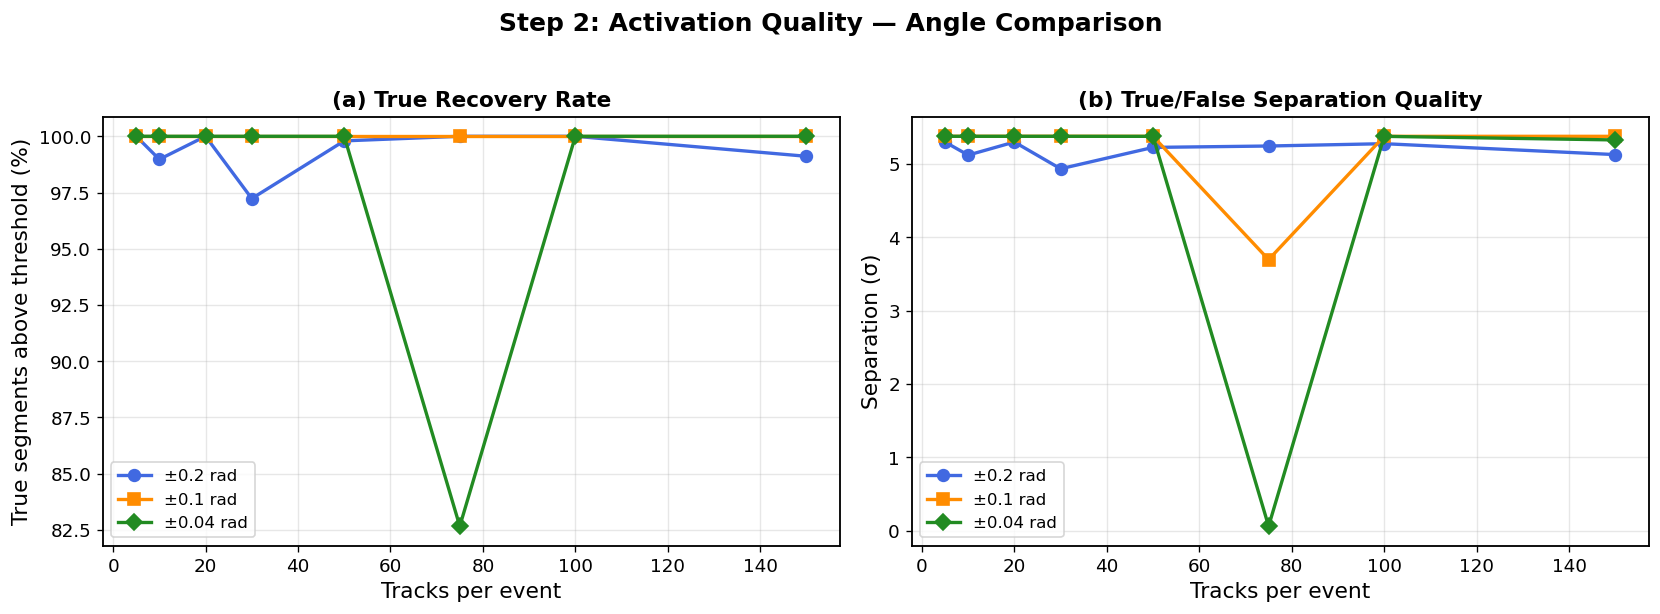
\includegraphics[width=0.85\textwidth]{step2_activation_summary.png}
  \caption{Step~2 summary plots.
    \emph{Left}: fraction of true segments recovered above threshold vs.\ track
    multiplicity.
    \emph{Right}: true\,/\,false separation quality (pooled Cohen's $d$).
    The severe dip for $\pm0.04$\,rad at 75 tracks is clearly visible in both
    panels.}
  \label{fig:step2_summary}
\end{figure}

\begin{figure}[htbp]
  \centering
  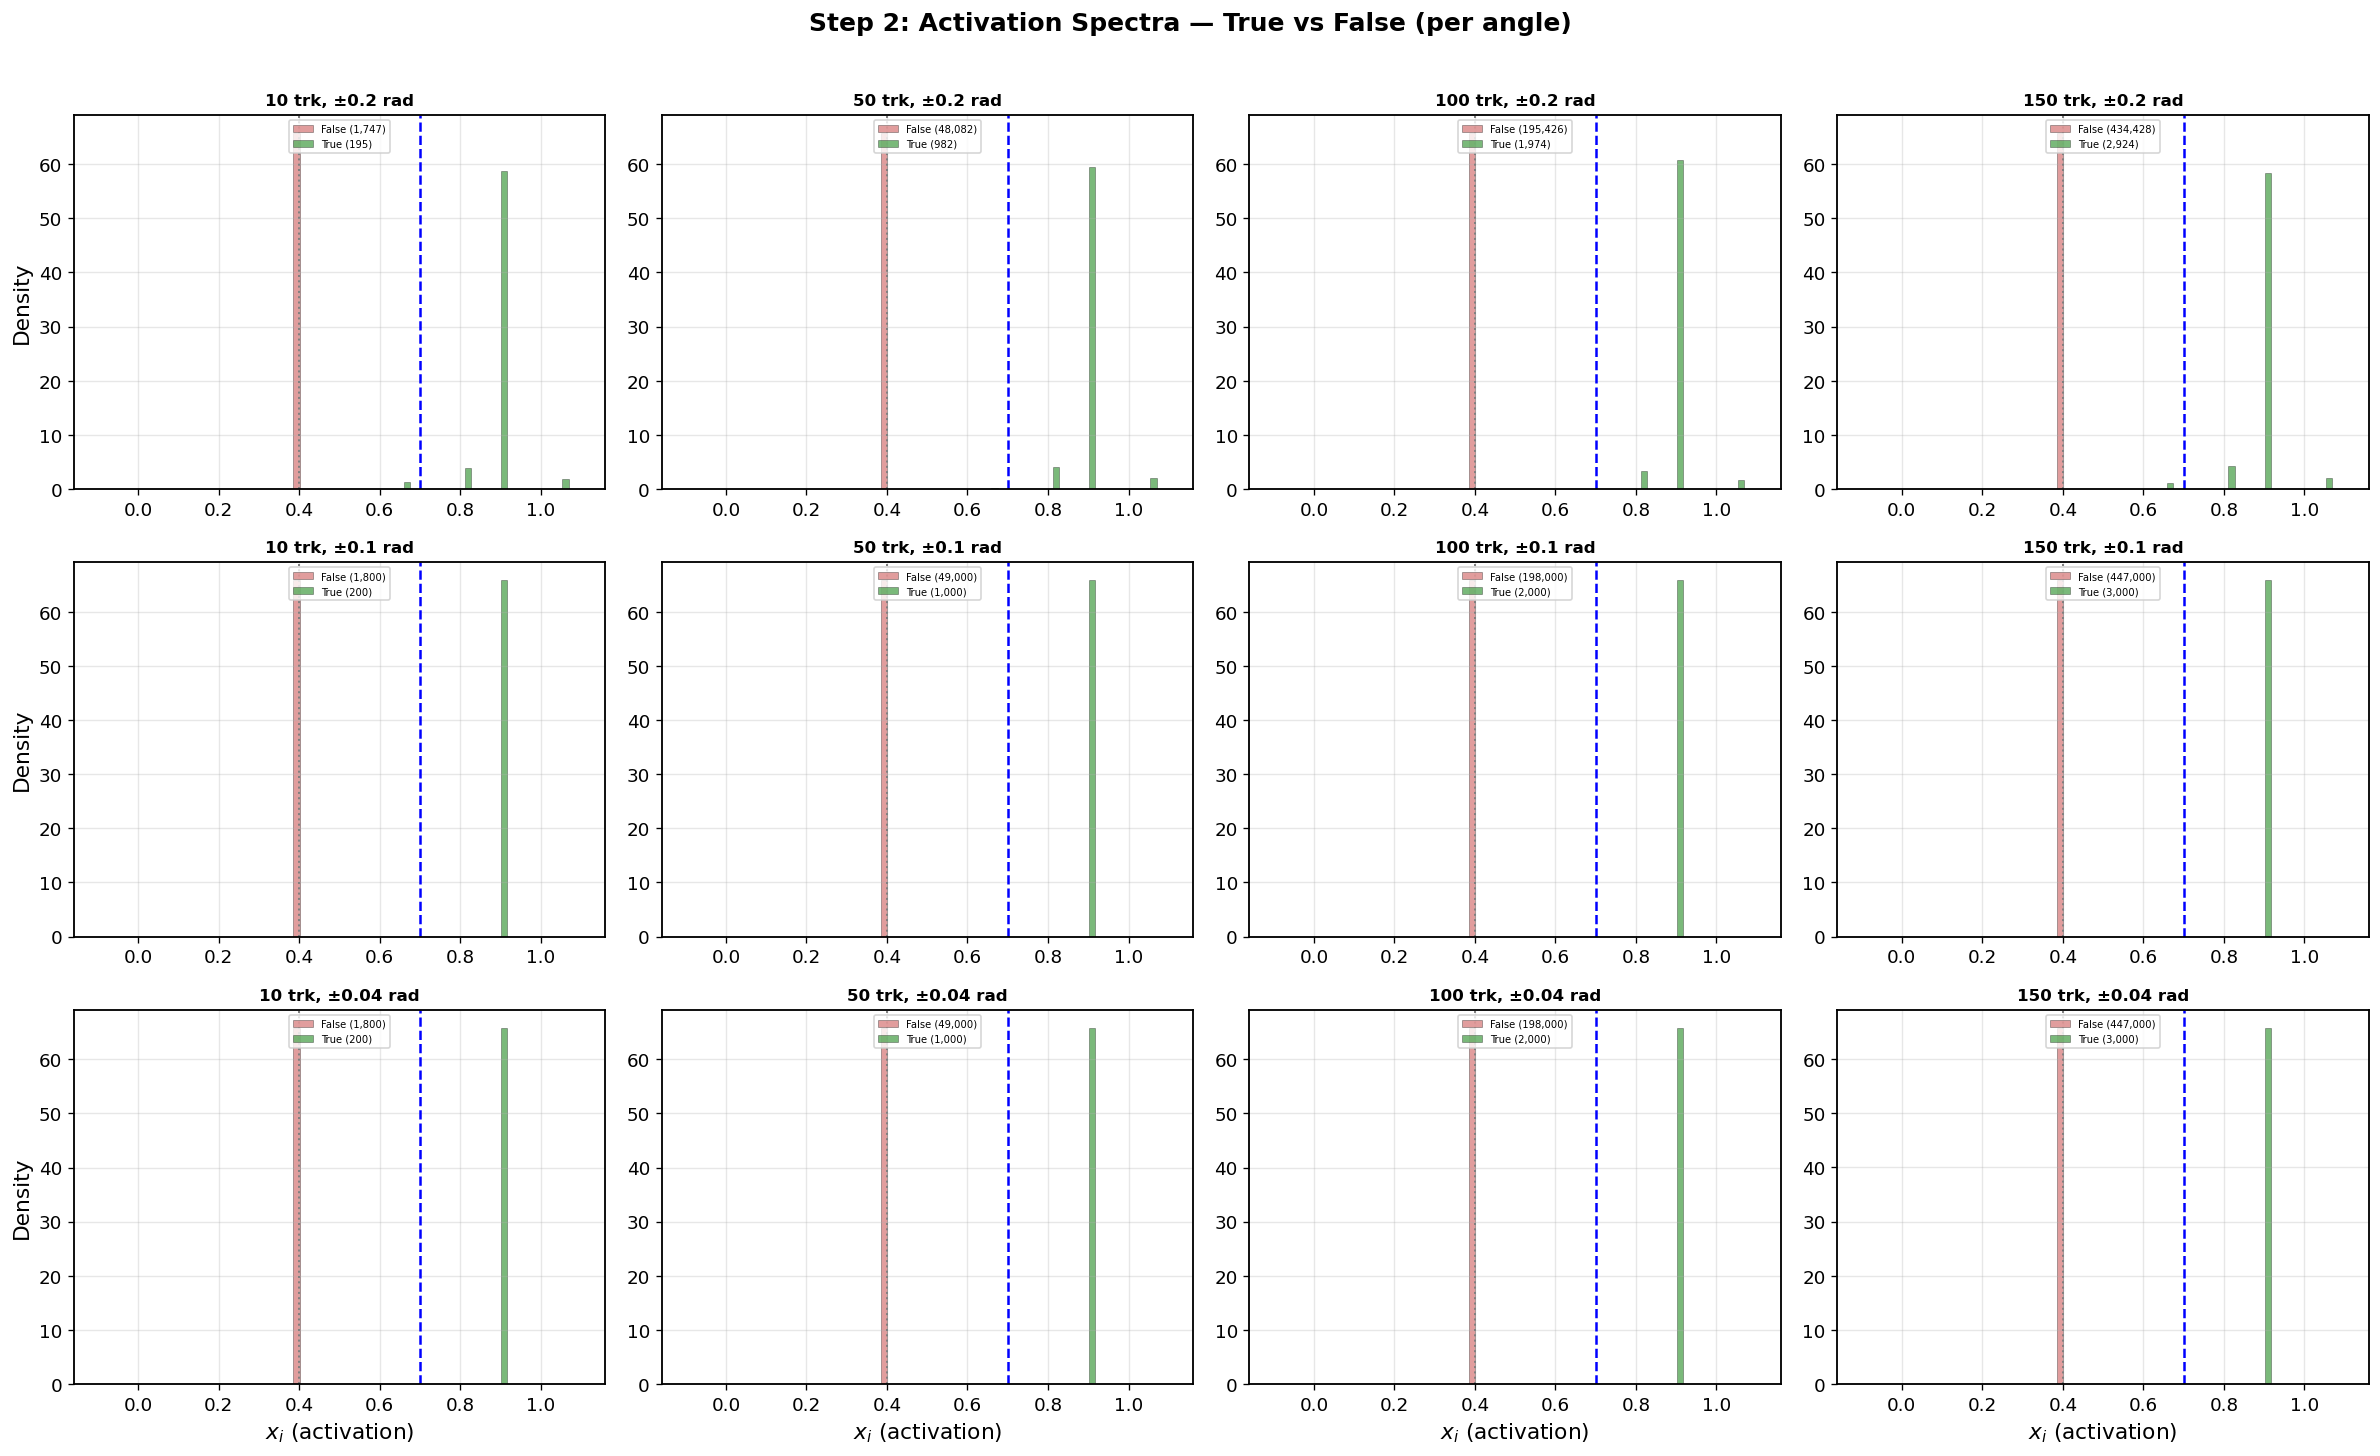
\includegraphics[width=0.9\textwidth]{step2_activation_spectra.png}
  \caption{Activation spectra (Step~2) for all three angle settings at
    selected track multiplicities.
    Green = true segments; red = false segments.
    The extreme spread of the true-segment distribution for $\pm0.04$\,rad
    at 75 tracks is clearly visible in the corresponding histogram panel.
    All other panels show well-separated bimodal distributions.}
  \label{fig:step2_spectra}
\end{figure}

% =============================================================================
\section{Theoretical Background: Condition Numbers and Gershgorin Discs}
\label{sec:theory}

Before analysing the root cause, we establish the mathematical framework
that underpins the diagnosis.

\subsection{The Condition Number}
\label{sec:theory_kappa}

Given a linear system $A\mathbf{x} = \mathbf{b}$, the \emph{condition number}
$\kappa(A)$ quantifies how much a small perturbation $\delta\mathbf{b}$ in the
right-hand side can be amplified into a perturbation $\delta\mathbf{x}$ in
the solution:
\begin{equation}
  \frac{\|\delta\mathbf{x}\|}{\|\mathbf{x}\|}
  \;\leq\; \kappa(A)\;\frac{\|\delta\mathbf{b}\|}{\|\mathbf{b}\|}.
  \label{eq:kappa_bound}
\end{equation}
For real symmetric matrices (which includes the Hamiltonian~$A$),
the 2-norm condition number is the ratio of the largest to smallest
eigenvalue in absolute value:
\begin{equation}
  \kappa_2(A) = \frac{|\lambda_\text{max}|}{|\lambda_\text{min}|}.
  \label{eq:kappa_eig}
\end{equation}
More generally, the condition number is defined via the singular value
decomposition $A = U\Sigma V^T$:
\begin{equation}
  \kappa(A) = \frac{\sigma_1}{\sigma_n},
  \label{eq:kappa_svd}
\end{equation}
where $\sigma_1 \geq \cdots \geq \sigma_n > 0$ are the singular values.
For a symmetric positive-definite matrix, $\sigma_i = \lambda_i$ and both
definitions coincide.
For indefinite matrices, $\sigma_i = |\lambda_i|$ and the SVD-based
$\kappa$ is the only well-defined measure.

\paragraph{Interpretation.}
$\kappa \approx 1$ means the solution is insensitive to perturbations.
$\kappa \sim 10^k$ means roughly $k$ digits of precision are lost.
$\kappa \to \infty$ means the matrix is singular.

\paragraph{Iterative solver convergence.}
For the Conjugate Gradient algorithm on a symmetric positive-definite
system, the relative error after $k$ iterations satisfies\footnote{G.H.\ Golub \& C.F.\ Van Loan, \emph{Matrix Computations}, 4th ed., Johns Hopkins, 2013.}
\begin{equation}
  \frac{\|\mathbf{x}_k - \mathbf{x}^*\|_A}
       {\|\mathbf{x}_0 - \mathbf{x}^*\|_A}
  \;\leq\; 2\left(\frac{\sqrt{\kappa} - 1}{\sqrt{\kappa} + 1}\right)^{\!k}.
  \label{eq:cg_convergence}
\end{equation}
This bound holds \textbf{only for SPD matrices}.
When the matrix is indefinite, the CG algorithm has no convergence
guarantee and can diverge or converge to a wrong solution.

\subsection{Gershgorin's Circle Theorem}
\label{sec:theory_gershgorin}

\begin{theorem}[Gershgorin, 1931]
Every eigenvalue of a matrix $A \in \mathbb{R}^{n\times n}$ lies within at
least one of the $n$ \emph{Gershgorin discs}
\begin{equation}
  D_i = \bigl\{\, z \in \mathbb{C} \;:\; |z - A_{ii}| \leq R_i \,\bigr\},
  \qquad
  R_i = \sum_{j \neq i} |A_{ij}|,
  \label{eq:gershgorin}
\end{equation}
where $A_{ii}$ is the diagonal entry (\emph{centre}) and $R_i$ is the sum
of absolute values of all off-diagonal entries in row~$i$ (\emph{radius}).
\end{theorem}

\noindent Two important corollaries follow directly:

\begin{corollary}[Strict diagonal dominance $\Rightarrow$ non-singularity]
If $|A_{ii}| > R_i$ for every row~$i$, then no Gershgorin disc contains
the origin, so $A$ is non-singular.
Moreover, if all diagonal entries share the same sign, $A$ is
\emph{definite}.
\end{corollary}

\begin{corollary}[Indefiniteness test]
If all diagonal entries share the same sign and $R_i > |A_{ii}|$ for at least
one row~$i$, then the corresponding disc crosses the origin.
If other discs remain on the same side, the matrix has
eigenvalues of both signs and is \textbf{indefinite}.
\end{corollary}

\subsection{Application to the Hamiltonian}
\label{sec:theory_hamiltonian}

\paragraph{Sign convention.}
The code internally constructs a raw matrix with negative diagonal
$-(\delta+\gamma)$ and positive off-diagonal couplings $+1$, then stores
$\hat{A} = -A_\text{raw}$ as \texttt{self.A}.
All computations and plots use the \emph{stored} matrix, which has
\textbf{positive diagonal} and \textbf{negative off-diagonal} entries:
\begin{equation}
  A_{ij} = \begin{cases}
    +(\delta + \gamma) & \text{if } i = j, \\[3pt]
    -1 & \text{if segments } i,j \text{ share a middle hit and }
         \theta_{ij} < \varepsilon, \\[3pt]
    0  & \text{otherwise.}
  \end{cases}
  \label{eq:hamiltonian_entries}
\end{equation}
With the current parameters $\delta = 1.0$, $\gamma = 1.5$, each diagonal
entry is $A_{ii} = +2.5$ and each off-diagonal coupling is $A_{ij} = -1$.

\paragraph{Isolated track ($n_\text{seg} = 4$).}
Inter-segment couplings form a tridiagonal-like structure; each segment
shares at most 2 middle hits, so interior rows have $R_i = 2$ and end rows
have $R_i = 1$.
Since $|A_{ii}| = 2.5 > R_i^{\max} = 2$, strict diagonal dominance holds.
The Gershgorin discs span $[+0.5,\,+4.5]$ — safely in the positive
half-plane — and the condition number of this block is
$\kappa \leq 4.5/0.5 = 9$.

\paragraph{Two well-separated tracks.}
The matrix is block-diagonal, with each $4\times4$ block inheriting
diagonal dominance.
The full matrix $\kappa$ equals that of the worst-conditioned block
($\kappa \approx 5$).

\paragraph{Two near-coincident tracks
($\Delta\phi_\text{eff} < \varepsilon/f_\text{amp}$).}
Cross-segment couplings appear.
A hit shared by both tracks can couple to cross-segments from the other
track; the worst-case row acquires up to 2 additional off-diagonal entries
on top of the 2 same-track couplings, giving $R_i \leq 4$.
Since $|A_{ii}| = 2.5 < 4$, diagonal dominance is \textbf{violated}.
The affected disc becomes
\begin{equation}
  D_i = [+2.5 - 4,\;\; +2.5 + 4] = [-1.5,\;\; +6.5],
  \label{eq:disc_coupled}
\end{equation}
which crosses the origin.
A negative eigenvalue then becomes possible, and the matrix can become
indefinite.

We define a \emph{critical Gershgorin ratio} for each row,
\begin{equation}
  \rho_i = \frac{R_i}{|A_{ii}|} = \frac{\sum_{j \neq i}|A_{ij}|}{\delta + \gamma},
  \label{eq:gershgorin_ratio}
\end{equation}
which summarises the spectral health of the system:
\begin{center}
\begin{tabular}{lccc}
  \toprule
  Regime & $\rho_\text{max}$ & Definiteness & $\kappa$ \\
  \midrule
  Isolated tracks & $0.8$ & Pos.-definite & $\sim$$5\text{--}9$ \\
  Boundary        & $\approx 1$ & Marginal     & $\sim$$10\text{--}50$ \\
  Near-coincident & $>1$ (up to $1.6$) & \textbf{Indefinite} & Spikes \\
  \bottomrule
\end{tabular}
\end{center}

\noindent In Section~\ref{sec:kappa_mechanism} we verify this theoretical
framework numerically.
Figure~\ref{fig:gershgorin_visual} provides a visual companion to the
analysis above, contrasting the matrix structure and Gershgorin discs for
a well-separated event (top row) and a near-coincident event (bottom row).

\begin{figure}[htbp]
  \centering
  \IfFileExists{fig_theory_gershgorin_visual.png}{%
    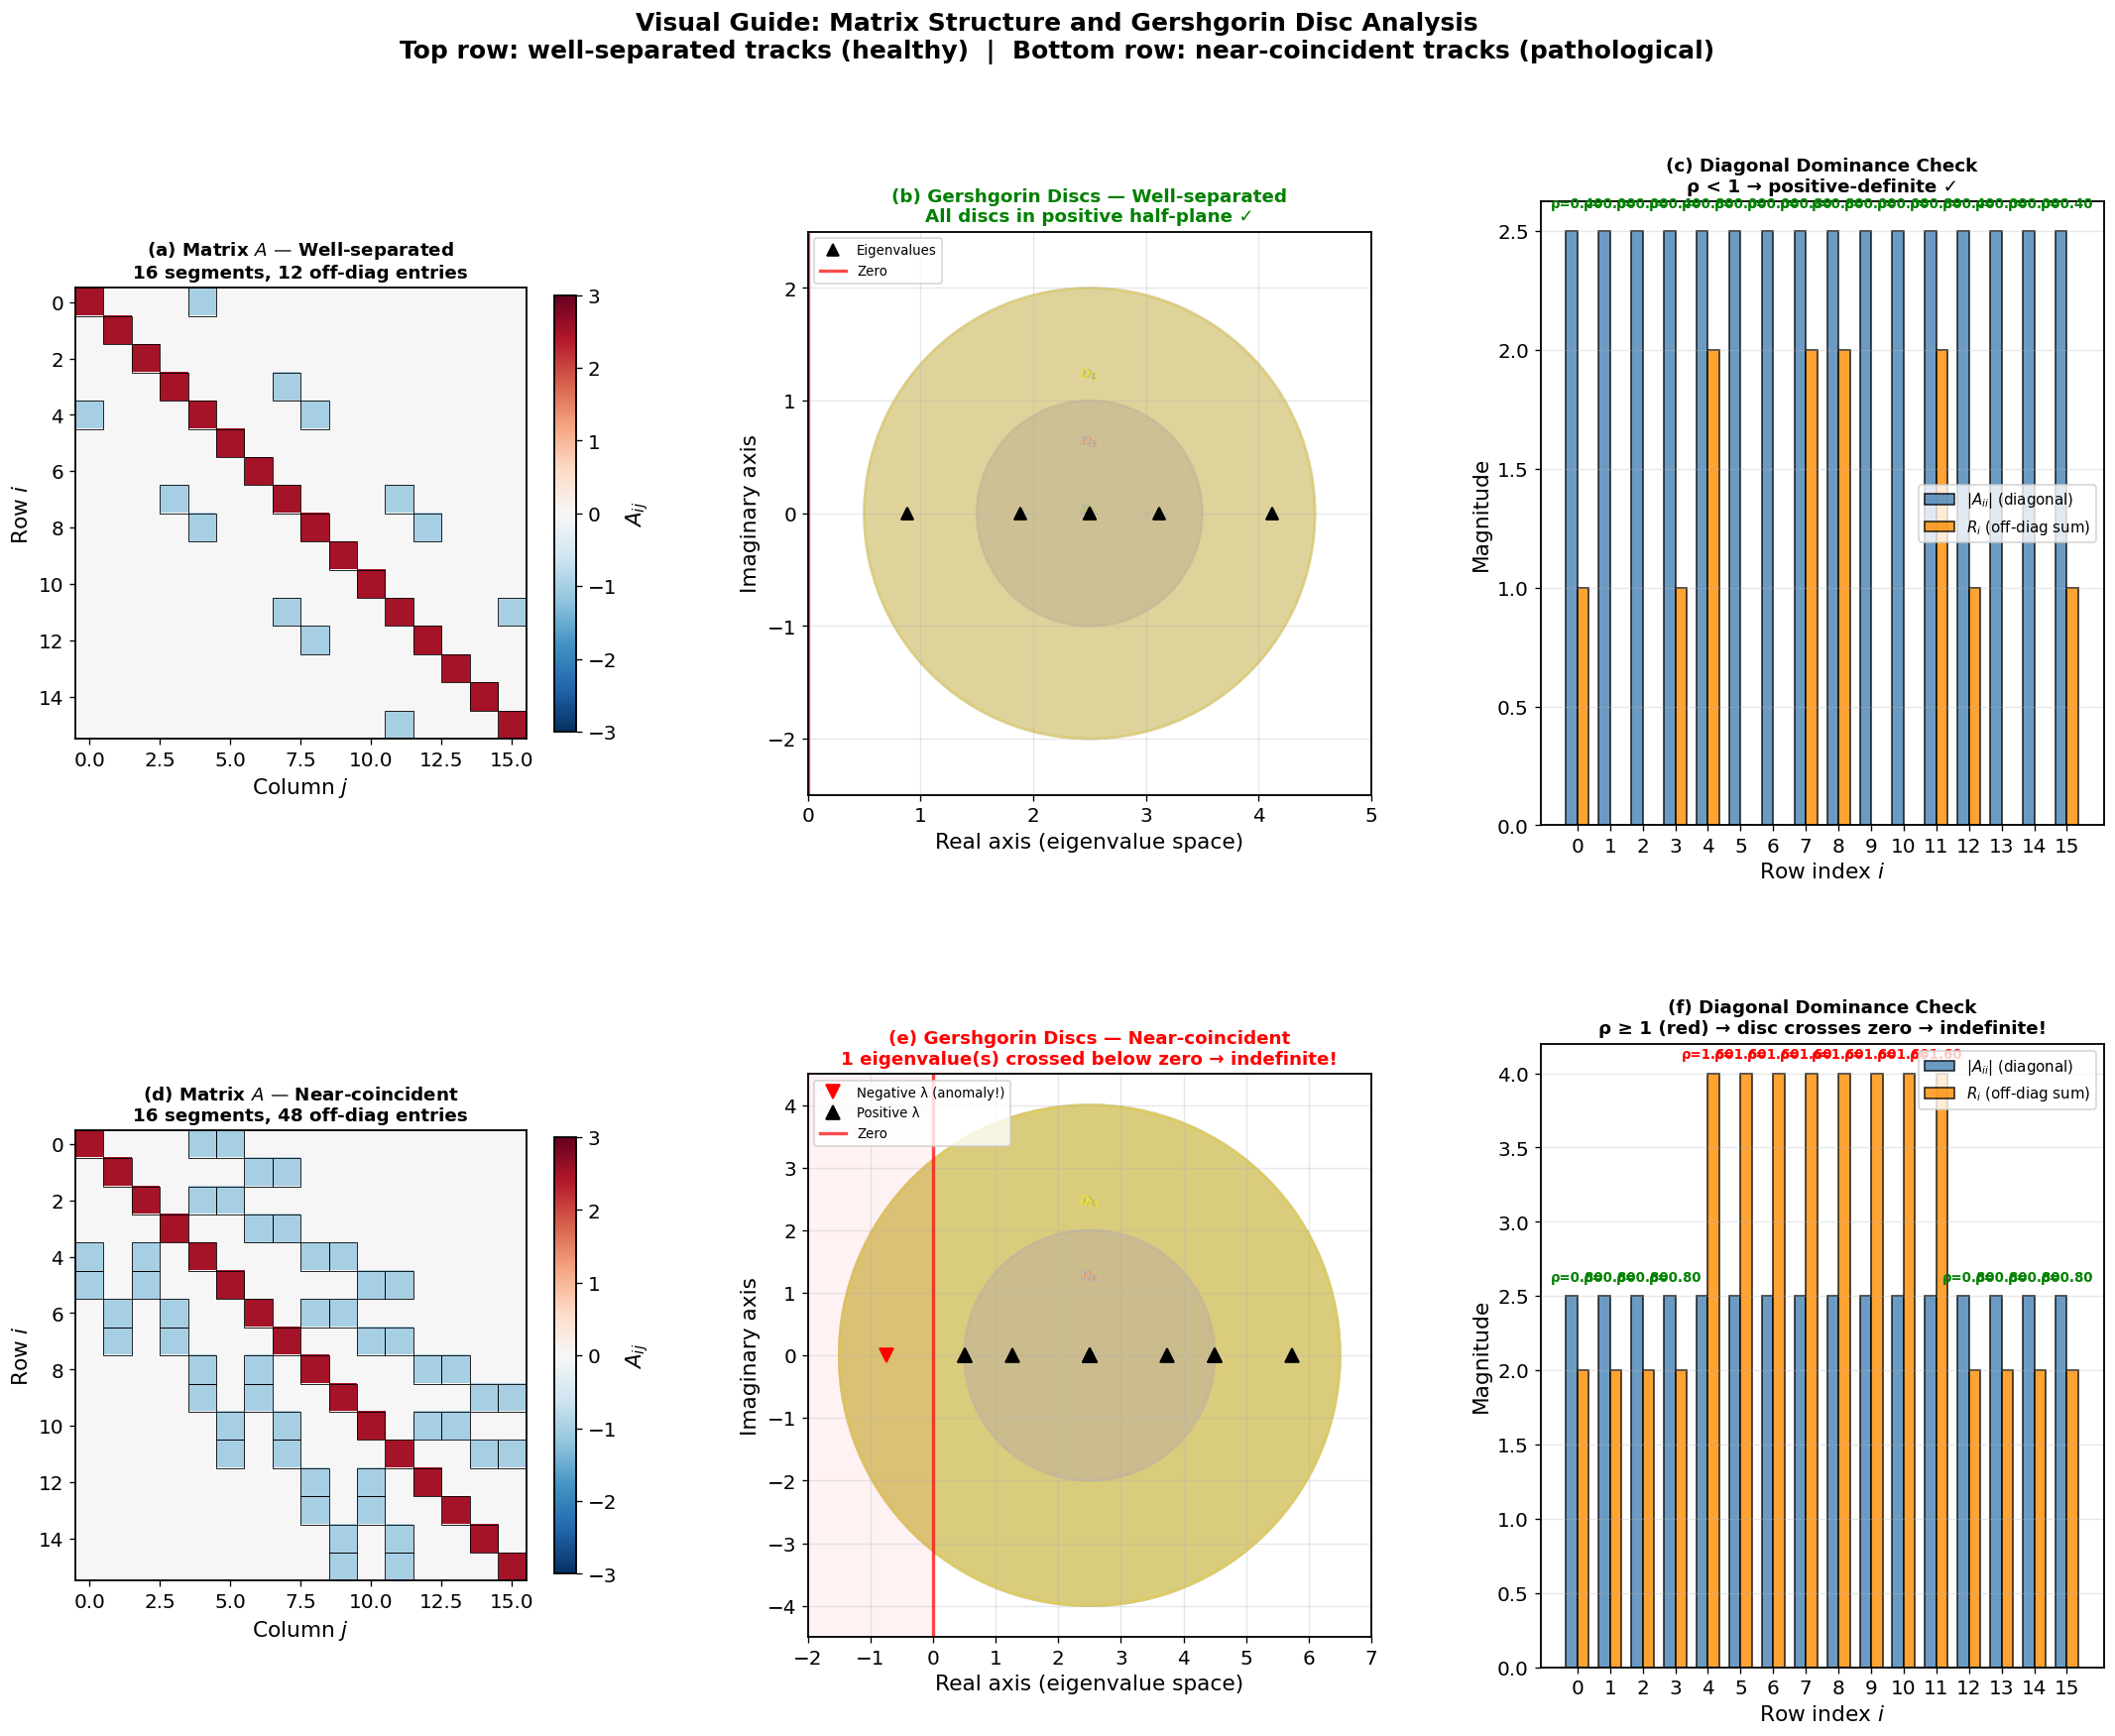
\includegraphics[width=\textwidth]{fig_theory_gershgorin_visual.png}}{%
    \fbox{\parbox{\textwidth}{\centering\vspace{2cm}fig\_theory\_gershgorin\_visual.png\\(re-run notebook to generate)\vspace{2cm}}}}
  \caption{Visual guide to matrix structure and Gershgorin disc analysis.
    \emph{Top row}: well-separated 2-track event --- (a)~block-diagonal matrix
    with 12 off-diagonal entries, (b)~Gershgorin discs safely within the positive
    half-plane, (c)~diagonal dominance satisfied ($\rho_i < 1$ for all rows).
    \emph{Bottom row}: near-coincident 2-track event --- (d)~dense cross-coupling
    (48 off-diagonal entries), (e)~enlarged discs crossing zero with one
    negative eigenvalue (red~$\triangledown$), (f)~diagonal dominance violated
    ($\rho_i \geq 1$, red labels), confirming indefiniteness.}
  \label{fig:gershgorin_visual}
\end{figure}

% =============================================================================
\section{Root Cause: Near-Coincident Track Degeneracy}
\label{sec:rootcause}

\subsection{Cross-Segment Angle Amplification}
\label{sec:amplification}

Consider two tracks $A$ and $B$ with angular parameters
$(\phi_A,\theta_A)$ and $(\phi_B,\theta_B)$, both originating from a
primary vertex near $z_0 = 50$\,mm.
A \emph{cross-segment} combines a hit from track~$A$ at module $k$ with a hit
from track~$B$ at module $k\!+\!1$ (or vice-versa).
The pairwise angle between the \emph{incoming} true segment for~$A$
(from module $k\!-\!1$ to $k$) and the \emph{outgoing} cross-segment
(from $A$'s hit at $k$ to $B$'s hit at $k\!+\!1$) is, to leading order in
small angles,
\begin{equation}
  \theta_\text{cross}^{(k)} \;\approx\;
  \frac{z_k - z_0}{z_{k+1} - z_k}\,
  \sqrt{(\phi_A - \phi_B)^2 + (\theta_A - \theta_B)^2},
  \label{eq:cross_angle}
\end{equation}
where $z_k$ is the $z$-position of module $k$ and $z_0$ is the primary
vertex $z$.
For the toy geometry ($z_0=50$\,mm, module $z$-positions
$\{100, 133, 166, 199, 232\}$\,mm, $\Delta z = 33$\,mm), the amplification
factor at the middle module ($z_3 = 166$\,mm) is the largest:
\begin{equation}
  f_\text{amp} = \frac{166 - 50}{33} \approx 3.5.
  \label{eq:famp}
\end{equation}
A cross-segment is accepted into the Hamiltonian whenever
$\theta_\text{cross} < \eps = 0.425$\,mrad, i.e.\ when
\begin{equation}
  \Delta\phi_\text{eff}
  \equiv \sqrt{(\phi_A-\phi_B)^2 + (\theta_A-\theta_B)^2}
  < \frac{\eps}{f_\text{amp}} \approx \frac{0.425\,\text{mrad}}{3.5}
  \approx 0.12\,\text{mrad}.
  \label{eq:tolerance}
\end{equation}

\subsection{Segment Construction and the Coupling Criterion}
\label{sec:segment_construction}

To understand why the threshold~\eqref{eq:tolerance} exists, one must
understand exactly how the Hamiltonian builds its matrix.  The process has
two stages, and the threshold emerges naturally from their interaction.

\paragraph{Stage 1: Cartesian segment generation.}
The Hamiltonian does \emph{not} know which track produced which hit.
For every pair of adjacent modules $(M_k, M_{k+1})$, it forms the
\textbf{Cartesian product} of all hits on~$M_k$ with all hits
on~$M_{k+1}$, generating one candidate segment per pair.  With $n$ tracks
and one hit per track per module, each module pair produces $n^2$ segments:
$n$~true (same-track) and $n(n-1)$ cross-track candidates.

For a concrete 2-track example (tracks $A$ and $B$), the four segments
between modules $k$ and $k\!+\!1$ are:
\begin{center}
\begin{tabular}{lccc}
  \toprule
  Segment & Start hit & End hit & Type \\
  \midrule
  $s_1$ & $a_k$     & $a_{k+1}$ & True (track~$A$) \\
  $s_2$ & $b_k$     & $b_{k+1}$ & True (track~$B$) \\
  $s_3$ & $a_k$     & $b_{k+1}$ & \textbf{Cross} ($A \to B$) \\
  $s_4$ & $b_k$     & $a_{k+1}$ & \textbf{Cross} ($B \to A$) \\
  \bottomrule
\end{tabular}
\end{center}

\noindent Cross-segments always exist in the segment list regardless of
track separation.  What matters is whether they get \emph{coupled} in the
matrix --- this is determined by Stage~2.

\paragraph{Stage 2: Pairwise coupling via the angle test.}
Two segments $i$ and $j$ receive an off-diagonal matrix entry
$A_{ij} = -1$ only if \textbf{both} of the following conditions are met:
\begin{enumerate}
  \item \textbf{Shared middle hit.}  The end hit of segment~$i$ must be
    the \emph{same physical hit} (same unique identifier, same $(x,y,z)$
    coordinates) as the start hit of segment~$j$.
    This means they chain through a single spatial point.
    Crucially, hit~$a_k$ (belonging to track~$A$) and hit~$b_k$
    (belonging to track~$B$) at the same module are \emph{different
    objects} with different positions --- they do \emph{not} satisfy this
    condition, even if the tracks are very close.
  \item \textbf{Angle test.}  The angle between the direction vectors of
    segments~$i$ and~$j$ must satisfy $\theta_{ij} < \eps$.
\end{enumerate}

\paragraph{How the cross-path kink angle is determined.}
Consider the chain of two segments sharing hit~$a_k$:
\begin{equation}
  \underbrace{a_{k-1} \to a_k}_{\text{true segment (track }A\text{)}}
  \;\longrightarrow\;
  \underbrace{a_k \to b_{k+1}}_{\text{cross-segment (}A \to B\text{)}}.
  \label{eq:cross_chain}
\end{equation}
The first segment points along track $A$'s direction.  The second
deviates because $b_{k+1}$ belongs to track~$B$, which is offset from
track~$A$ by $\Delta\phi_\text{eff}$ in angular space.  The geometric
lever arm from the primary vertex magnifies this angular offset into a
kink angle $\theta_\text{cross} \approx f_\text{amp}\,\Delta\phi_\text{eff}$
at the junction point~$a_k$.

The two regimes are:
\begin{itemize}
  \item \textbf{Well-separated tracks}
    ($f_\text{amp}\,\Delta\phi_\text{eff} \gg \eps$):
    the kink angle far exceeds~$\eps$; condition~(2) rejects the pairing;
    no spurious coupling enters the matrix.  The matrix remains
    block-diagonal.
  \item \textbf{Near-coincident tracks}
    ($f_\text{amp}\,\Delta\phi_\text{eff} < \eps$):
    the kink angle is small enough that the angle test \emph{cannot
    distinguish} the cross-path from a true segment chain.  The coupling
    is accepted, injecting additional $-1$ entries into the matrix.
\end{itemize}

\noindent The critical separation threshold
$\Delta\phi_\text{eff}^\text{crit} = \eps / f_\text{amp}^{\max}$
is therefore not an arbitrary parameter: it is the
\textbf{angular resolution limit} of the Hamiltonian's coupling criterion.
Below this threshold, the matrix structure changes qualitatively from
block-diagonal (healthy) to cross-coupled (pathological).

\subsection{Why Two Tracks Suffice}
\label{sec:two_tracks}

A common misconception is that this effect requires many tracks piling up
in the same angular region.  In fact, the mechanism is \textbf{pairwise}:

\begin{enumerate}
  \item A single pair of tracks within $\Delta\phi_\text{eff} < 0.12$\,mrad
    is sufficient to inject cross-couplings.
  \item In the worst case (2 tracks, 5 modules), each same-track segment
    can couple to up to 2 cross-segments in addition to its 2 same-track
    neighbours, raising the maximum Gershgorin radius from $R_i = 2$ to
    $R_i = 4$.
  \item Since the diagonal entry is $A_{ii} = \delta + \gamma = 2.5 < 4$,
    diagonal dominance is violated and the matrix becomes indefinite ---
    with just 2 tracks.
\end{enumerate}

\noindent More tracks in the same angular window make the problem worse
(each additional near-coincident track adds further off-diagonal entries,
increasing~$R_i$ and deepening the indefiniteness).
However, the \emph{fundamental mechanism} already operates with a single
pair.  This explains why the observed anomaly is triggered by a single
stochastic near-coincident pair in a 75-track event, rather than requiring
a large cluster of coincident tracks.

\subsection{Probability of a Near-Coincident Pair}
\label{sec:probability}

For tracks drawn uniformly from a square cone of half-angle $\phi_\text{max}$
in both $\phi$ and $\theta$, the angular area is $A_\text{cone} =
(2\phi_\text{max})^2$.
The probability that \emph{any specific pair} of tracks falls within the
mutual angular distance $\Delta\phi_\text{eff} < 0.12$\,mrad is
\begin{equation}
  p_\text{pair} = \frac{\pi\,(0.12\,\text{mrad})^2}{(2\phi_\text{max})^2}
  = \frac{\pi \times 1.44\times10^{-8}}{16\,\phi_\text{max}^2}.
  \label{eq:ppair}
\end{equation}
The expected number of near-coincident pairs in an event with $n=75$ tracks is
\begin{equation}
  \langle N_\text{degen}\rangle
  = \binom{75}{2}\,p_\text{pair}
  = 2775\,p_\text{pair}.
  \label{eq:ndegen}
\end{equation}
Table~\ref{tab:prob} shows the values for all three angle settings.

\begin{table}[h!]
  \centering
  \caption{Expected degenerate pairs at $n=75$ tracks per event, and the
    cumulative probability of at least one such pair appearing in 5 repeat
    events.}
  \label{tab:prob}
  \begin{tabular}{lrrr}
    \toprule
    Angle setting & $p_\text{pair}$ & $\langle N_\text{degen}\rangle$ per event &
    $P(\geq1\text{ in }5\text{ events})$ \\
    \midrule
    $\pm0.2$\,rad & $8.5 \times 10^{-8}$ & $2.4\times10^{-4}$ & $0.1\%$ \\
    $\pm0.1$\,rad & $3.4 \times 10^{-7}$ & $9.5\times10^{-4}$ & $0.5\%$ \\
    $\pm0.04$\,rad & $2.1 \times 10^{-6}$ & $5.9\times10^{-3}$ & $2.9\%$ \\
    \bottomrule
  \end{tabular}
\end{table}

\noindent At $\pm0.04$\,rad there is therefore a $\sim$$3\%$ chance that
at least one of the 5 repeat events contains a near-coincident pair.
This is consistent with the observed anomaly appearing in exactly one of
the studied density points.

\subsection{Effect on the Linear System}
\label{sec:matrix_effect}

When two tracks $A$ and $B$ satisfy $\Delta\phi_\text{eff} < 0.12$\,mrad,
the Hamiltonian acquires additional off-diagonal couplings linking
\emph{cross-segments} to true segments.
Denote the four true segments for track~$A$ by
$\{a_1, a_2, a_3, a_4\}$ and for track~$B$ by $\{b_1, b_2, b_3, b_4\}$.
Normally, these form two independent $4\times4$ sub-systems.
With spurious cross-segment couplings, the sub-system expands to
an $8\times8$ block with mixed off-diagonal entries, whose structure
depends on how many cross-segment angles satisfy $\theta_\text{cross}<\eps$.

In the limiting case where $A$ and $B$ are \emph{exactly} coincident
($\phi_A = \phi_B$, $\theta_A = \theta_B$), every cross-segment has
$\theta_\text{cross} = 0$, so all cross combinations are accepted.
The hits of $A$ and $B$ at each module then occupy the same detector position,
producing an 8$\times$8 sub-matrix where many rows and columns are
\emph{identical} or linearly dependent.
This renders the matrix \textbf{rank-deficient or near-singular}.

\subsection{Structural Mechanism of the Condition Number Spike}
\label{sec:kappa_mechanism}

The chain of causation from small track separation to a spiking condition
number $\kappa$ can be decomposed into four distinct stages, each
illustrated in Figure~\ref{fig:kappa_mechanism}:

\begin{enumerate}
  \item \textbf{Off-diagonal coupling injection.}
    When $\Delta\phi_\text{eff} < \varepsilon / f_\text{amp}$,
    cross-segments linking hits from \emph{different} tracks are accepted
    into the Hamiltonian.  Each cross-segment adds $-1$ entries to
    off-diagonal positions in $\mathbf{A}$.
    Panel~(d) of Figure~\ref{fig:kappa_mechanism} shows the off-diagonal
    count increasing by a factor of~$\approx\!4\times$ as $\phi_\text{max}$
    falls below $\phi_\text{crit}$, consistent with the emergence of
    inter-track couplings.

  \item \textbf{Gershgorin disc widening.}
    For each row~$i$, the Gershgorin disc is centred at
    $A_{ii} = +(\delta+\gamma) = +2.5$ with radius
    $R_i = \sum_{j\neq i}|A_{ij}|$.
    Additional off-diagonal entries increase~$R_i$, widening the disc.
    Panel~(c) of Figure~\ref{fig:kappa_mechanism} directly compares the
    Gershgorin discs for a well-separated event (discs entirely within the
    positive half-plane) and a near-coincident event (discs crossing zero).

  \item \textbf{Sign flip and indefiniteness.}
    When $R_i > |A_{ii}|$ for any row, the corresponding Gershgorin disc
    crosses the origin, meaning an eigenvalue can flip sign (become negative).
    Panel~(e) quantifies this: the maximum row-level ratio
    $R_i / |A_{ii}|$ exceeds~$1$ for separations below
    $\sim\!0.15$\,mrad — exactly where indefiniteness appears.

  \item \textbf{Singular value spread.}
    An indefinite matrix whose eigenvalues span both signs tends to have
    a wider spread of singular values, increasing
    $\kappa = \sigma_\text{max}/\sigma_\text{min}$.
    Panel~(f) shows the direct correlation: events with more off-diagonal
    couplings systematically have higher condition numbers,
    with indefinite matrices (red crosses) occupying the upper-right region.
\end{enumerate}

\noindent Panels~(a) and~(b) of Figure~\ref{fig:kappa_mechanism} provide
a direct structural comparison: the matrix heat-maps for well-separated
(12 off-diagonal entries, block-diagonal) versus near-coincident
(28 off-diagonal entries, dense inter-block couplings) events.
All condition number plots use \textbf{logarithmic scales} on both axes.

\begin{figure}[htbp]
  \centering
  \IfFileExists{fig4a_condition_number_mechanism.png}{%
    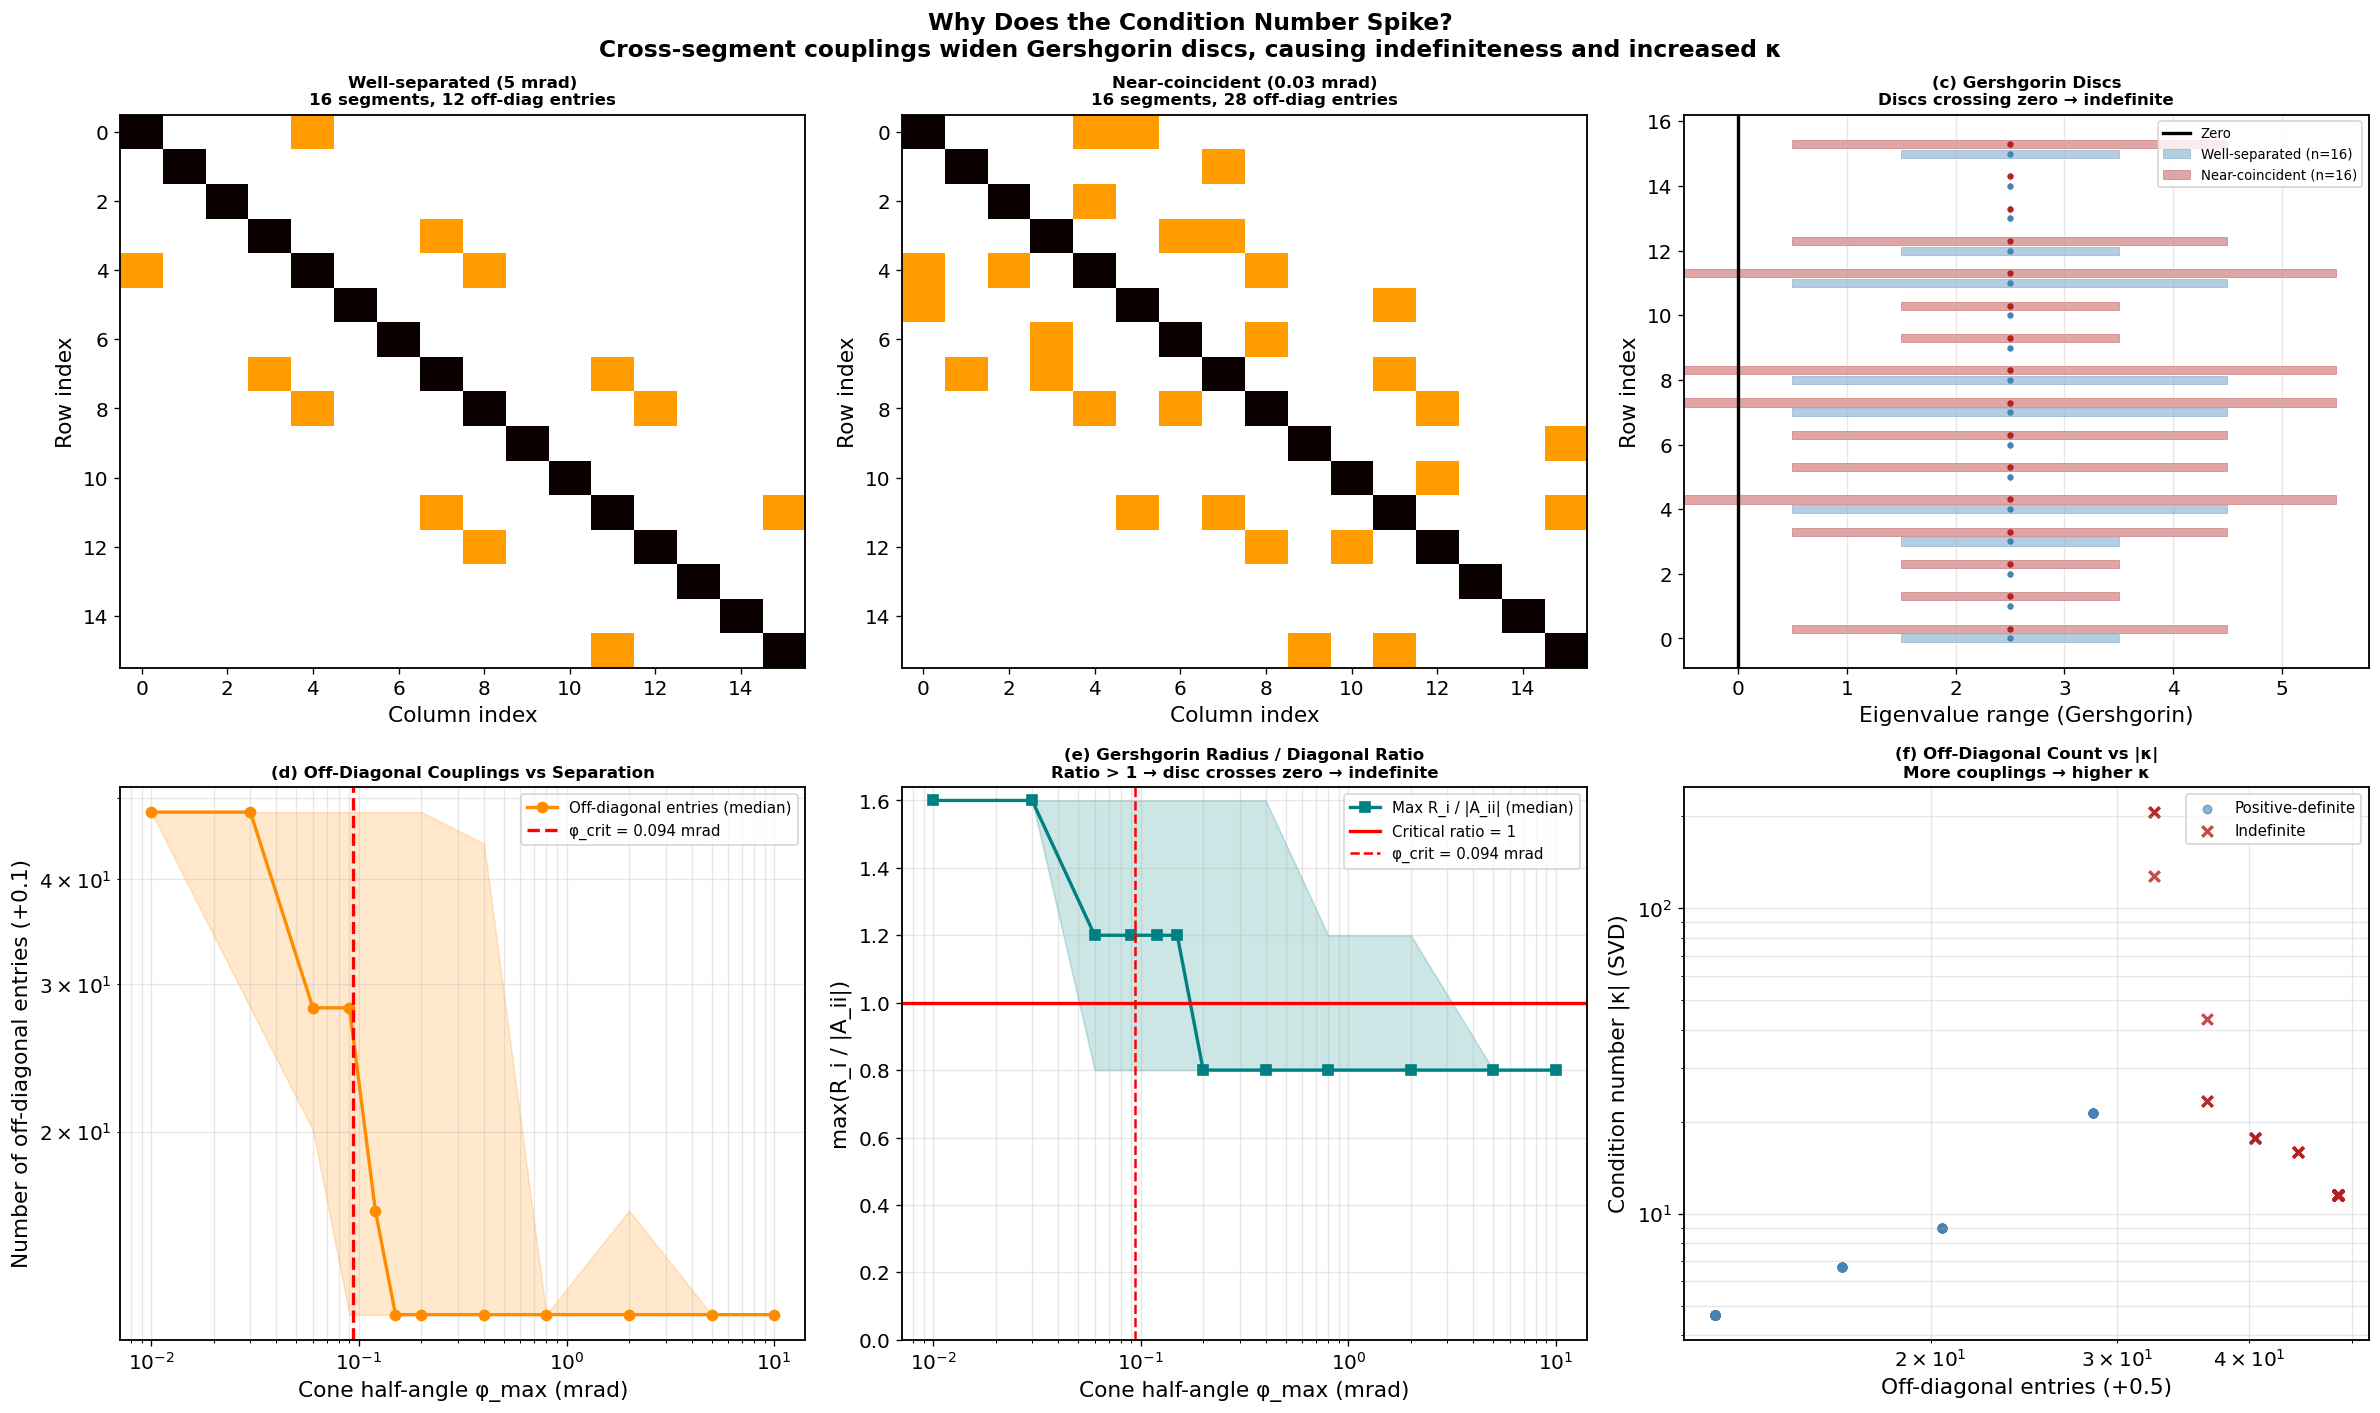
\includegraphics[width=\textwidth]{fig4a_condition_number_mechanism.png}}{%
    \fbox{\parbox{\textwidth}{\centering\vspace{2cm}fig4a\_condition\_number\_mechanism.png\\(re-run notebook to generate)\vspace{2cm}}}}
  \caption{Structural mechanism of the condition number spike.
    \emph{(a,\,b)}: Hamiltonian matrix heat-maps for well-separated and
    near-coincident 2-track events, showing the injection of off-diagonal
    cross-segment couplings.
    \emph{(c)}: Gershgorin discs — the near-coincident case (red) has discs
    crossing zero, indicating indefiniteness.
    \emph{(d)}: Off-diagonal count vs.\ track separation (log scale) —
    sharp increase below $\phi_\text{crit}$.
    \emph{(e)}: Maximum Gershgorin radius-to-diagonal ratio — exceeding~1
    is the necessary condition for indefiniteness.
    \emph{(f)}: Off-diagonal count vs.\ SVD condition number (log-log) —
    indefinite matrices (red $\times$) cluster at higher~$\kappa$.}
  \label{fig:kappa_mechanism}
\end{figure}

\subsection{Matrix Indefiniteness}
\label{sec:indefiniteness}

A critical finding of this analysis is that near-coincident track
configurations cause the Hamiltonian matrix $\mathbf{A}$ to become
\textbf{indefinite} — i.e.\ it acquires negative eigenvalues.
This is a more severe pathology than mere ill-conditioning:
the matrix fundamentally violates the positive-definiteness assumption
that underpins the Conjugate Gradient solver.

For a well-separated event the diagonal entries $A_{ii} = \delta + \gamma = 2.5$
dominate the off-diagonal couplings ($A_{ij} = -1$), and the Gershgorin disc
for each row stays entirely in the positive half of the real line.
However, when cross-segment couplings are injected, a row corresponding to
a hit shared by many accepted cross-segments can have a Gershgorin radius
that exceeds its diagonal entry, pushing the disc (and the corresponding
eigenvalue) below zero.

Numerical experiments show that for 2-track events with the
current parameters ($\gamma = 1.5$, $\delta = 1.0$):
\begin{itemize}
  \item At $\phi_\text{max} = 0.02$\,mrad (deep in the spurious regime):
    $100\%$ of events produce an indefinite matrix.
  \item At $\phi_\text{max} = 0.10$\,mrad: $\approx38\%$ are indefinite.
  \item At $\phi_\text{max} \geq 0.50$\,mrad: $<3\%$ are indefinite.
\end{itemize}
The correctly computed condition number (SVD-based, $|\kappa| = \sigma_\text{max}/\sigma_\text{min}$)
remains moderate ($|\kappa| \approx 7\text{--}30$) even for indefinite matrices.
The system is \emph{not} truly ill-conditioned; the matrix simply has the
wrong sign structure.

\paragraph{$\gamma$ sensitivity.}
The old reference code historically used $\gamma = 2.0$ (diagonal $= 3.0$),
compared with the current $\gamma = 1.5$ (diagonal $= 2.5$).
Higher~$\gamma$ strengthens the diagonal dominance and reduces the
frequency of indefiniteness — e.g.\ from $100\%$ to $\approx42\%$ at
$\phi_\text{max} = 0.02$\,mrad.
However, $\gamma = 2.0$ does \emph{not} guarantee positive definiteness at
very small separations.
A fully robust solution would require either (a) ensuring
$\gamma + \delta$ exceeds the maximum possible row sum of off-diagonal
magnitudes, or (b) switching to a solver that does not require SPD matrices.

\paragraph{Condition number measurement artefact.}
Earlier versions of the analysis reported $\kappa \sim 10^{12}\text{--}10^{15}$
using the naive formula $\kappa = \lambda_\text{max}/\max(\lambda_\text{min},\,\varepsilon)$.
This formula is only valid for positive-definite matrices.
When $\lambda_\text{min} < 0$, the guard $\max(\lambda_\text{min},\varepsilon)$
replaces the true minimum eigenvalue with $\varepsilon \sim 10^{-12}\text{--}10^{-15}$,
producing an artificially enormous $\kappa$.
The correct SVD-based condition number $|\kappa| = \sigma_1 / \sigma_n$ is well-defined
regardless of sign structure and reveals the system is \emph{not} ill-conditioned.
Figure~\ref{fig:kappa_comparison} shows the naive versus correct condition numbers.

\subsection{Conjugate Gradient Divergence}
\label{sec:cg_divergence}

The CG solver (\texttt{scipy.sparse.linalg.cg}, relative
tolerance $10^{-5}$, default \texttt{atol=0}) requires the system matrix to be
symmetric positive definite (SPD).
As shown in Section~\ref{sec:indefiniteness}, near-coincident track
configurations produce \textbf{indefinite} matrices which violate this
fundamental precondition.
This is potentially a significant concern: the CG solver has no convergence
guarantee on indefinite systems, and in practice produces arbitrarily wrong
results.

On indefinite systems the CG iterates can diverge or stagnate.
Scipy returns the current (unconverged) iterate, which manifests as:
\begin{itemize}
  \item Activations wildly outside $[0,1]$:
        observed range $[-75.1,\;+154.0]$ at $\pm0.04$\,rad, $n=75$.
  \item Standard deviation of true activations $\sigma_{x_\text{true}} = 6.04$
        (vs.\ $\approx0.03$ in normal operation).
  \item False activations slightly below the analytic baseline ($0.393 < 0.400$),
        because the global residual error redistributes across all segments.
  \item Separation metric $|{\langle x_t\rangle - \langle x_f\rangle}|/\sigma_\text{pooled}$
        collapses to $0.26/4.28 \approx 0.06\,\sigma$ (effectively zero).
\end{itemize}

\noindent Figure~\ref{fig:kappa_comparison} illustrates the activation
distribution for the anomalous $\pm0.04$\,rad, $n=75$ case alongside healthy
distributions.

\begin{figure}[htbp]
  \centering
  \IfFileExists{fig4_condition_number_sweep.png}{%
    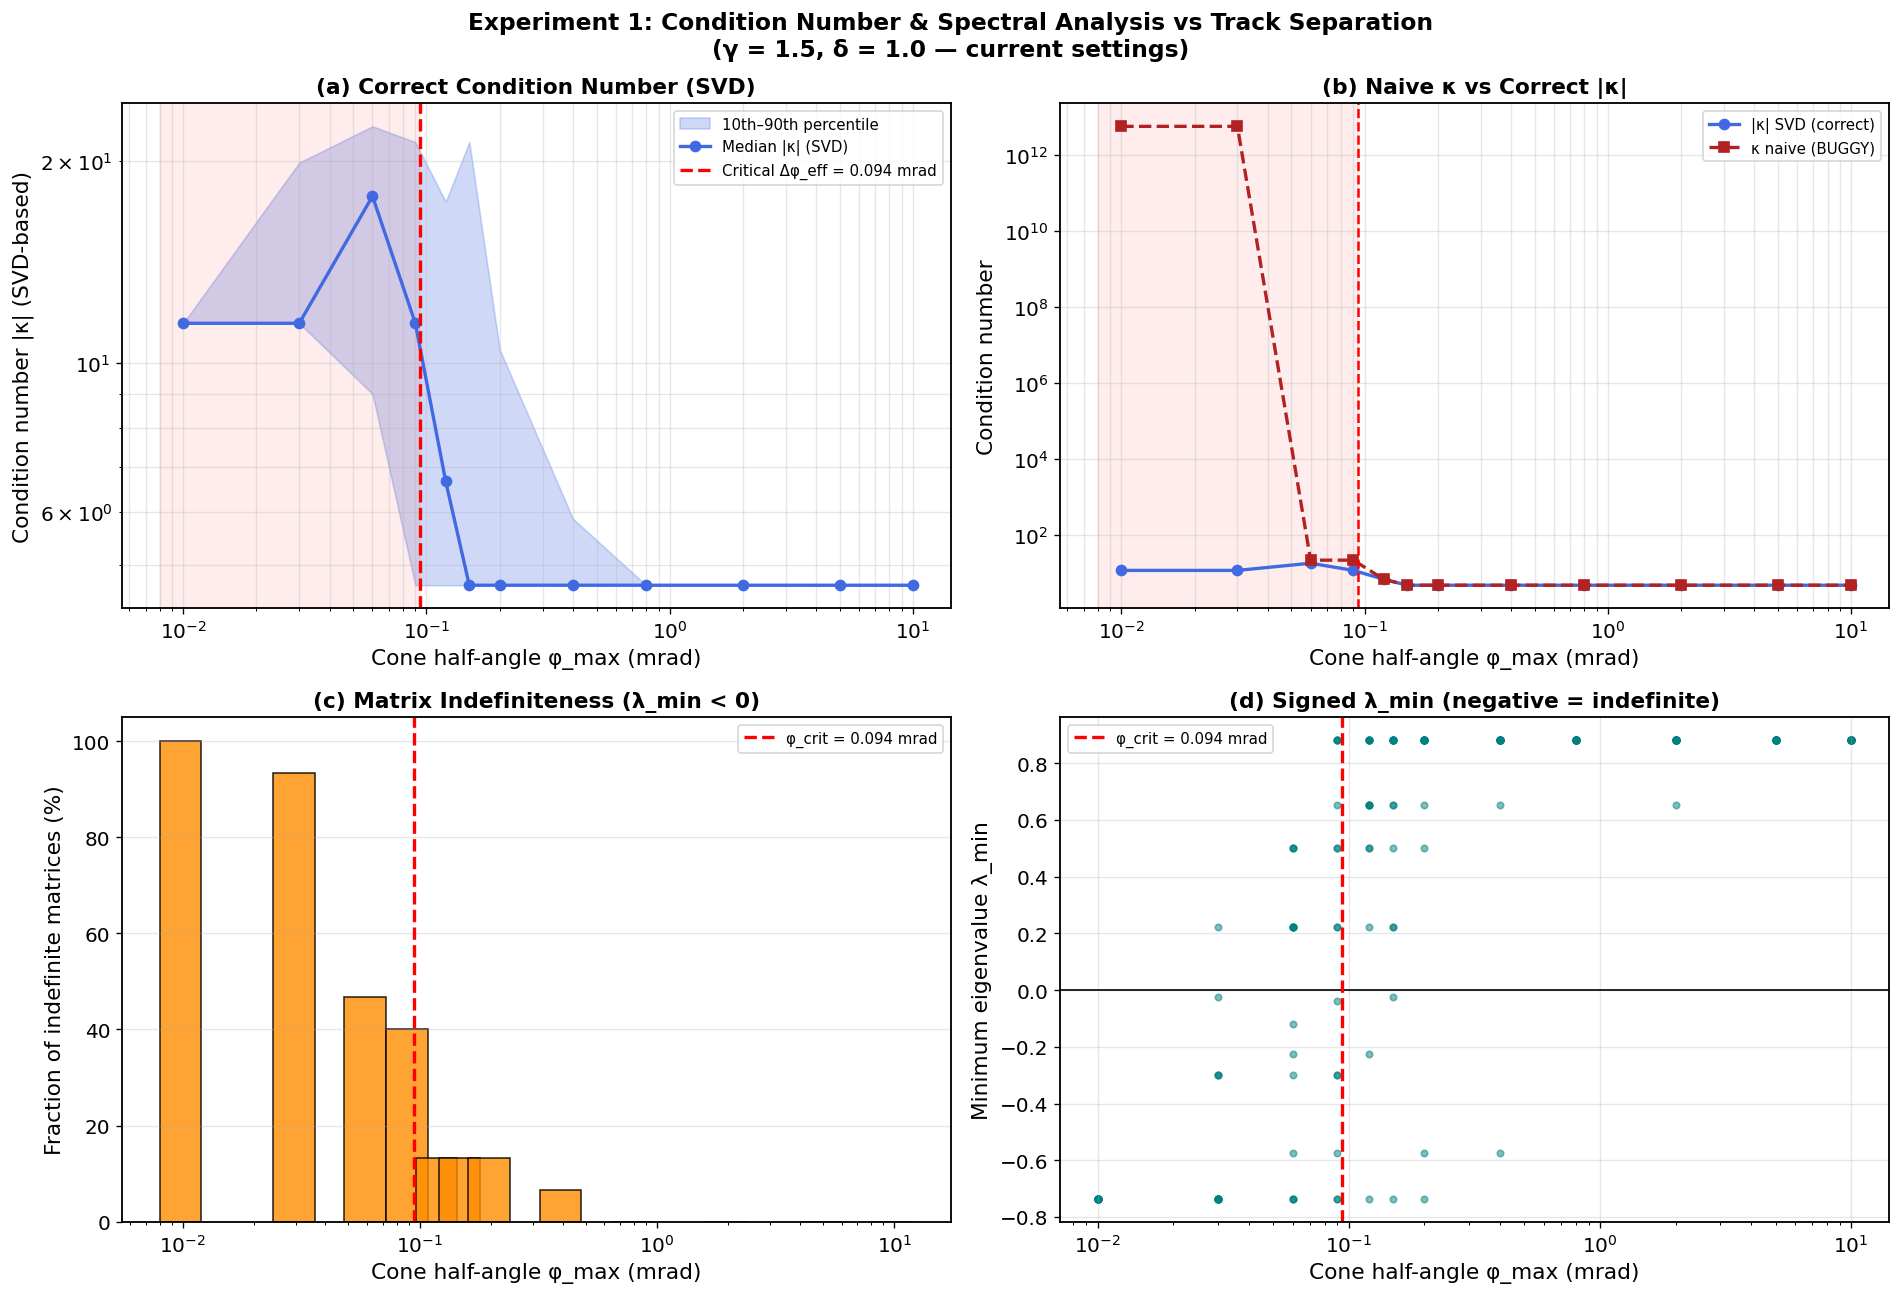
\includegraphics[width=0.9\textwidth]{fig4_condition_number_sweep.png}}{%
    \fbox{\parbox{0.9\textwidth}{\centering\vspace{2cm}fig4\_condition\_number\_sweep.png\\(re-run notebook to generate)\vspace{2cm}}}}
  \caption{Condition number analysis.
    \emph{Top left}: SVD-based condition number $|\kappa|$ vs.\ track separation.
    \emph{Top right}: naive $\kappa$ (old formula) vs.\ correct $|\kappa|$ ---
    the naive formula explodes by $\sim$$10^{12}$ for indefinite matrices while
    the correct value stays moderate.
    \emph{Bottom left}: fraction of indefinite matrices (negative $\lambda_\text{min}$).
    \emph{Bottom right}: signed minimum eigenvalue, showing negative values
    when tracks are within the critical separation.
    The discrepancy between naive and correct condition numbers is a
    measurement artefact, not a true ill-conditioning.}
  \label{fig:kappa_comparison}
\end{figure}

\begin{figure}[htbp]
  \centering
  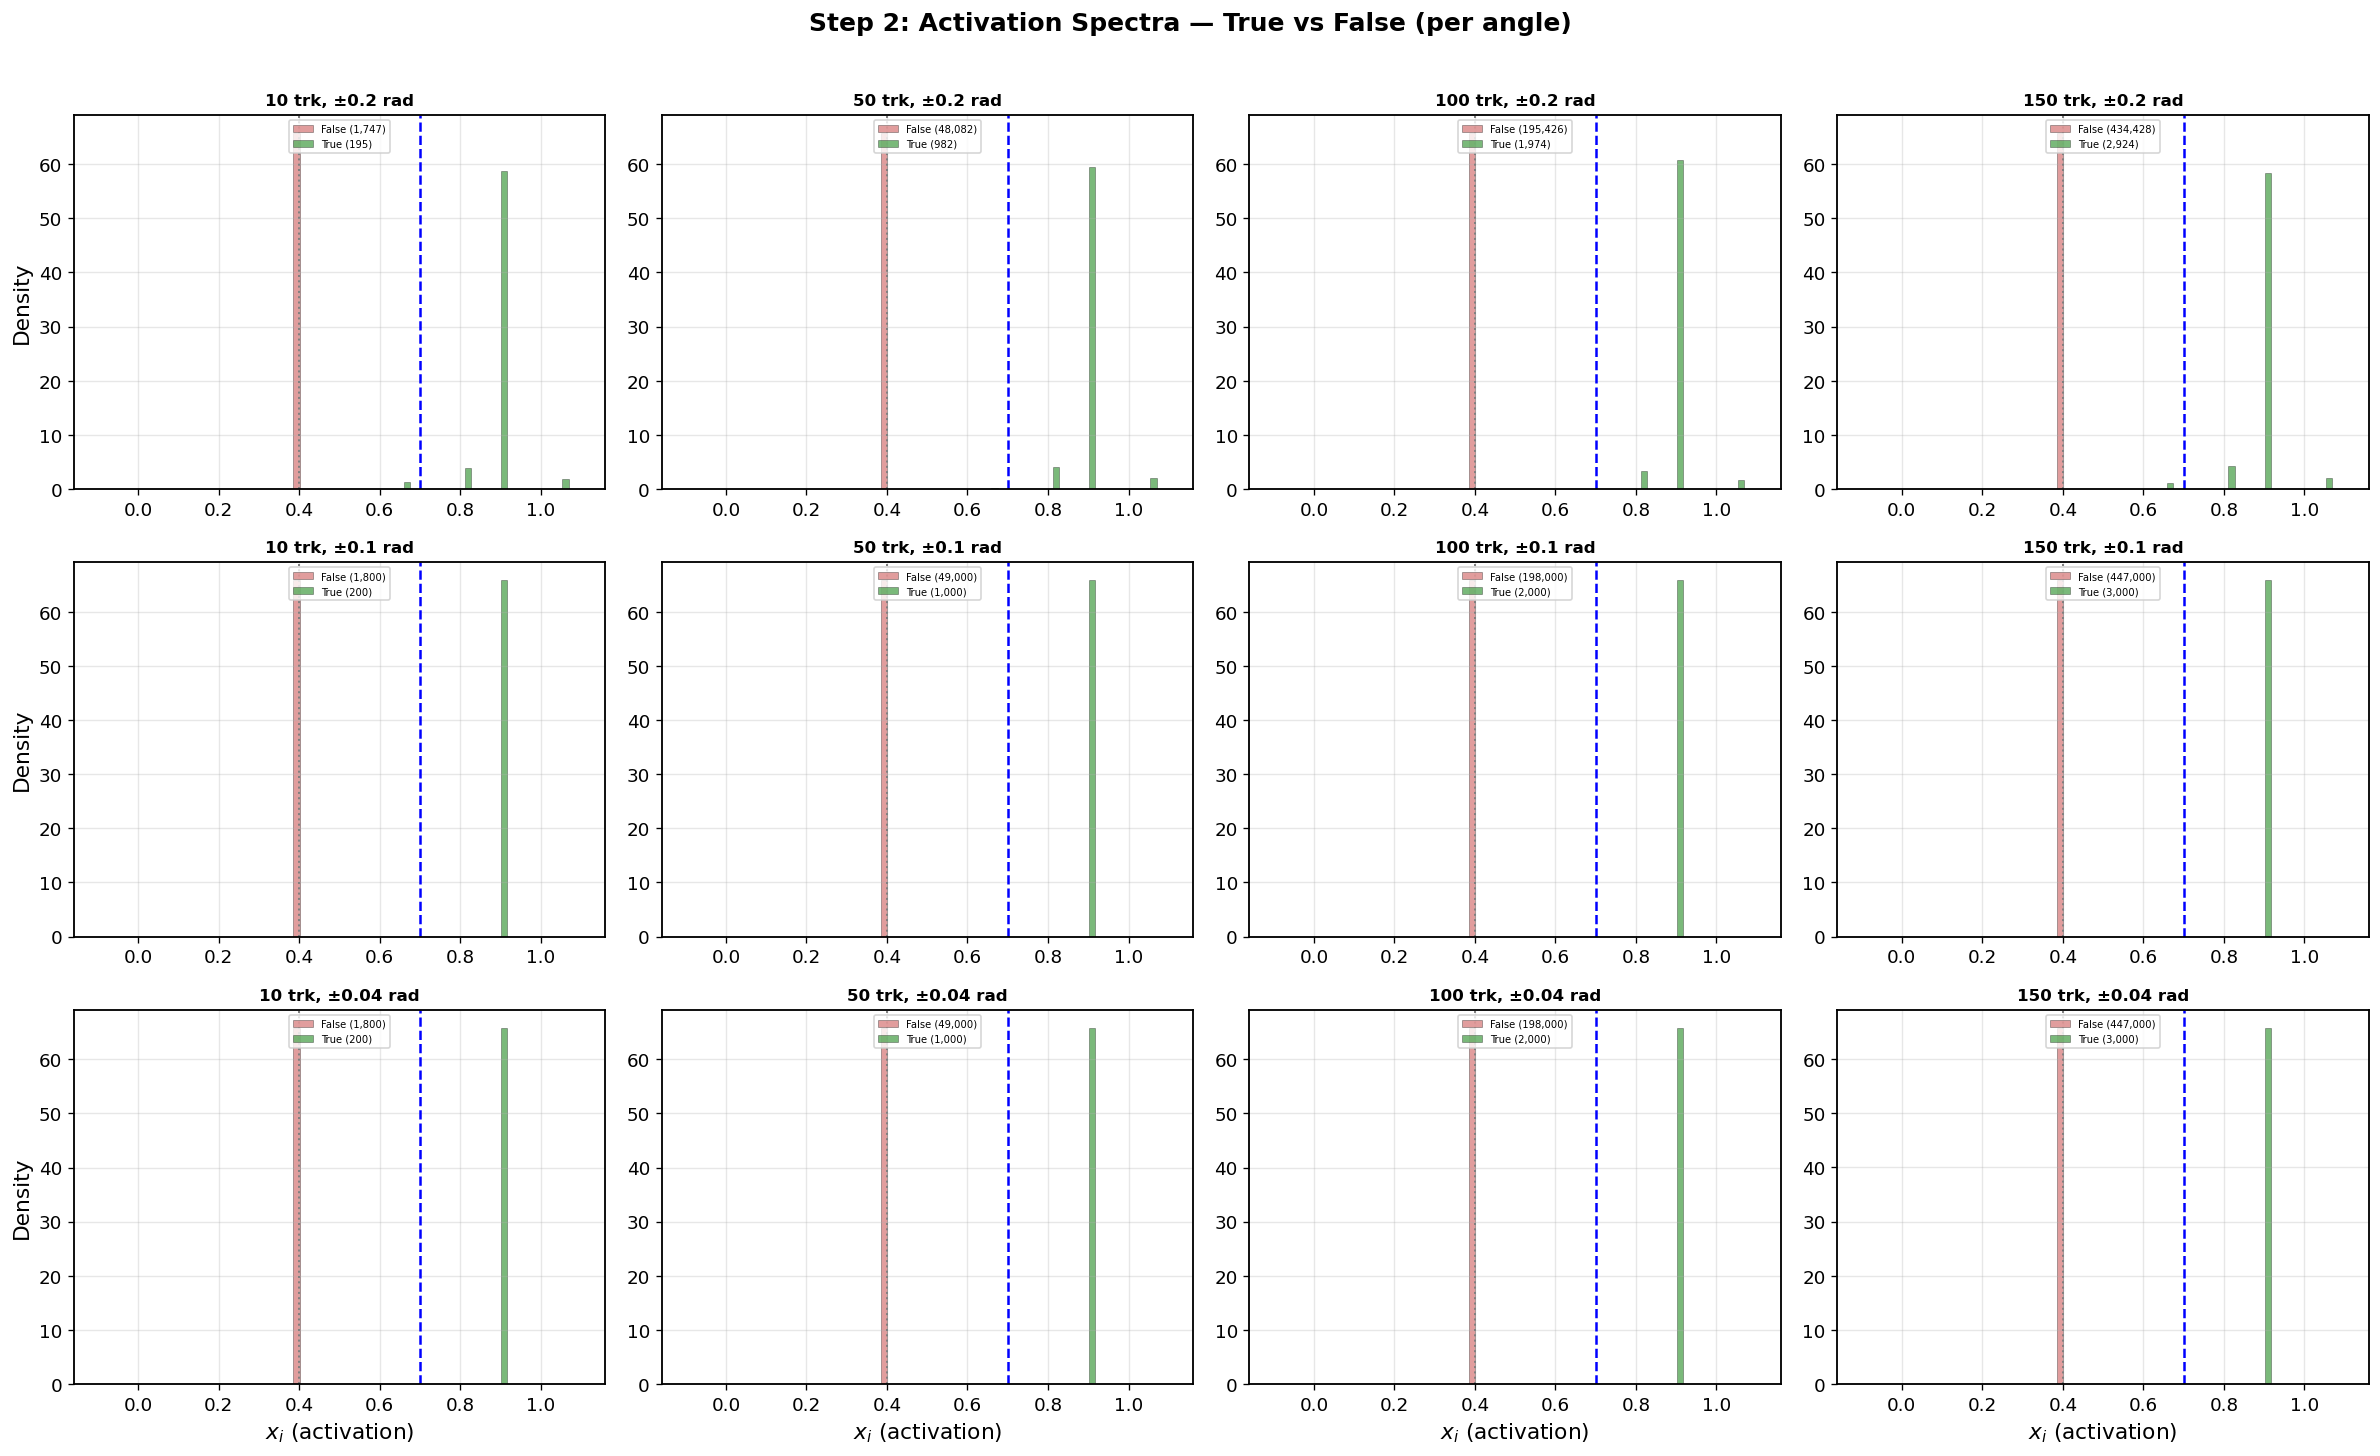
\includegraphics[width=0.9\textwidth]{step2_activation_spectra.png}
  \caption{Activation spectra comparing all three angle settings at
    selected track multiplicities.
    Green = true segments; red = false segments.
    The extreme spread of the true-segment distribution for $\pm0.04$\,rad
    at 75 tracks is clearly visible in the corresponding histogram panel.
    All other panels show well-separated bimodal distributions.}
  \label{fig:step2_spectra_full}
\end{figure}

\begin{figure}[htbp]
  \centering
  \IfFileExists{fig4c_gamma_sensitivity.png}{%
    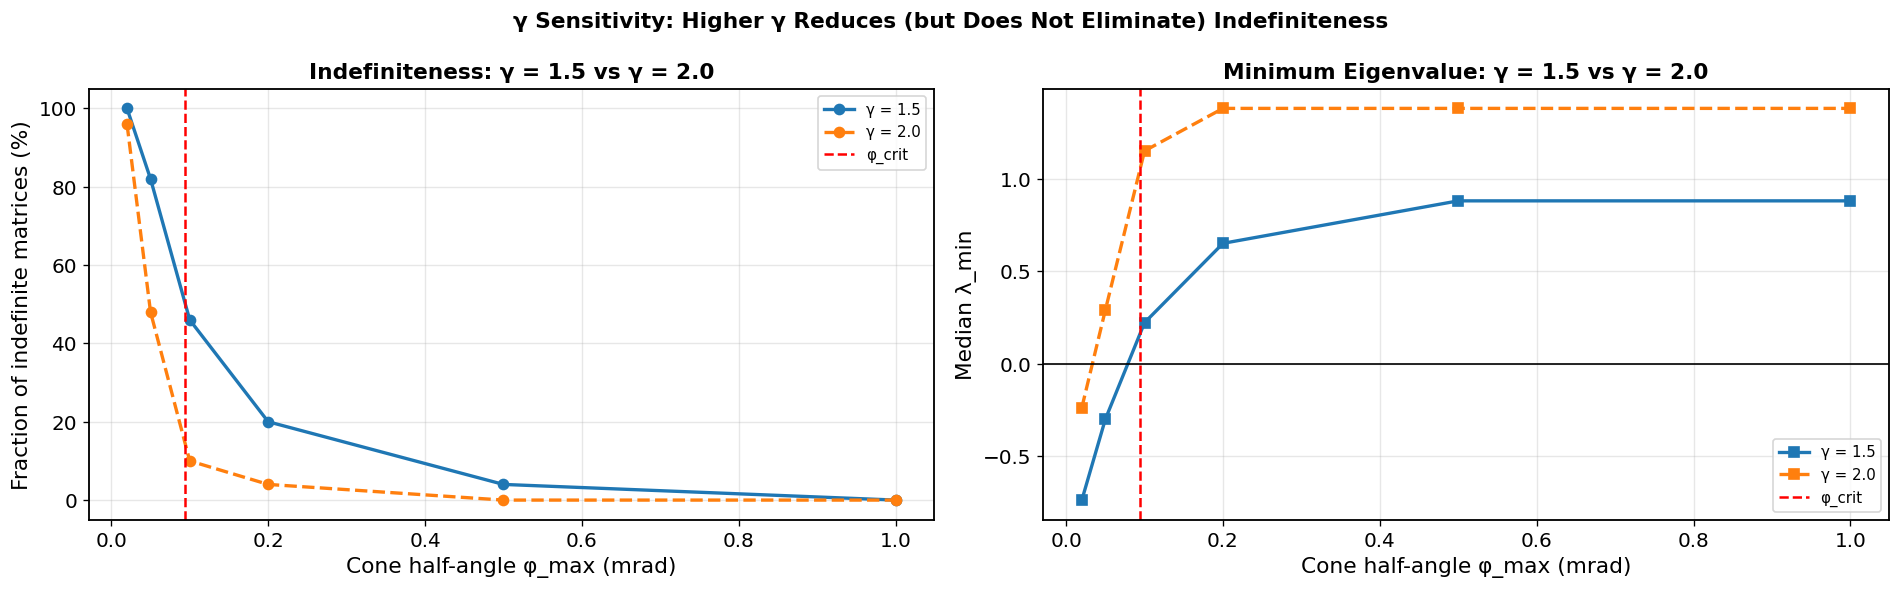
\includegraphics[width=0.85\textwidth]{fig4c_gamma_sensitivity.png}}{%
    \fbox{\parbox{0.85\textwidth}{\centering\vspace{2cm}fig4c\_gamma\_sensitivity.png\\(re-run notebook to generate)\vspace{2cm}}}}
  \caption{$\gamma$ sensitivity analysis.
    \emph{Left}: fraction of indefinite matrices for $\gamma = 1.5$ (current
    settings) vs.\ $\gamma = 2.0$ (old code).
    Higher $\gamma$ reduces indefiniteness by strengthening diagonal dominance,
    but does not eliminate it at very small separations ($< 0.05$\,mrad).
    \emph{Right}: median minimum eigenvalue $\lambda_\text{min}$ for both
    $\gamma$ values.}
  \label{fig:gamma_sensitivity}
\end{figure}

% =============================================================================
\section{Why the Dip is Localised at 75 Tracks}
\label{sec:localisation}

The anomaly appears at $n=75$ and \emph{not} at $n=50$ or $n=100$.
This is a consequence of three compounding factors:

\subsubsection*{(i) Small sample size ($N_\text{rep}=5$)}

With only 5 random events per density point, whether the anomaly appears
depends on whether the random number draws happen to produce a near-coincident
pair.
Given $P(\geq1\text{ in }5) \approx 3\%$ per density point, the expected
number of density points out of 8 that would show this pathology is
$0.03 \times 8 \approx 0.24$.
Finding exactly one such point (n=75) is therefore entirely consistent
with statistical expectation.
Had different random seeds been used, the anomaly could equally well
appear at $n=50$ or $n=100$ — or not at all.

\subsubsection*{(ii) Density-dependent probability}

Equation~\eqref{eq:ndegen} shows that $\langle N_\text{degen}\rangle \propto n$
(more tracks $\Rightarrow$ more pairs $\Rightarrow$ more chances for
coincidence).
Higher densities are therefore \emph{slightly} more susceptible, but the
effect is mild at these multiplicity values.

\subsubsection*{(iii) Angle-dependent track density}

Table~\ref{tab:prob} shows that the $\pm0.04$\,rad setting is
$\sim$$25\times$ more susceptible than $\pm0.2$\,rad.
This explains why neither $\pm0.2$ nor $\pm0.1$ exhibit the dip:
the probability per event is two orders of magnitude smaller,
effectively negligible in a 5-event sample.

% =============================================================================
\section{Step~3 Confirmation: Competition Analysis}
\label{sec:step3}

The Step~3 per-hit competition analysis runs on \emph{a fresh set of 5 events}
(independently generated from Step~2).
Its data for $\pm0.04$\,rad at $n=75$ tracks shows:
\begin{itemize}
  \item Mean true activation: $1.125$ (above the nominal 1.091).
  \item Mean false-competitor sum: $51.8 \approx 129.5 \times 0.4$
        (consistent with uncoupled false segments at baseline).
  \item Mean competitor count: $129.5$ (close to $175 - 1 = 174$ maximum possible).
\end{itemize}
These are all \emph{healthy} values, confirming that the Step~2 anomaly
was produced by a pathological configuration in that specific batch of
5 random seeds and did not reflect a systematic breakdown of the algorithm.

% =============================================================================
\section{Comparison Across Angle Settings}
\label{sec:comparison}

Table~\ref{tab:all_angles} provides the Step~2 metrics at 75 tracks for all
three generation angles.

\begin{table}[h!]
  \centering
  \caption{Step~2 metrics at $n=75$ tracks for all three angle settings.}
  \label{tab:all_angles}
  \begin{tabular}{lrrrr}
    \toprule
    Angle & $\langle x_\text{true}\rangle$ & Recovery (\%) & Separation ($\sigma$)
    & Max $|x_\text{false}|$ \\
    \midrule
    $\pm0.2$\,rad & 1.081 & 100.0 & 5.24 & 0.667 \\
    $\pm0.1$\,rad & 1.143 & 100.0 & 3.69 & 1.792 \\
    $\pm0.04$\,rad & \textbf{0.662} & \textbf{82.7} & \textbf{0.06} & $62.0$ \\
    \bottomrule
  \end{tabular}
\end{table}

\noindent A mild reduction in separation quality is also visible at $\pm0.1$\,rad
($3.69\,\sigma$ vs.\ the usual $5.37\,\sigma$), and the maximum false
activation reaches $1.79$ (compared with $0.67$ for $\pm0.2$).
This suggests a low-severity near-coincidence in one of the $\pm0.1$\,rad
events as well — without triggering solver divergence, but enough to
inject some spurious coupling.

\begin{figure}[htbp]
  \centering
  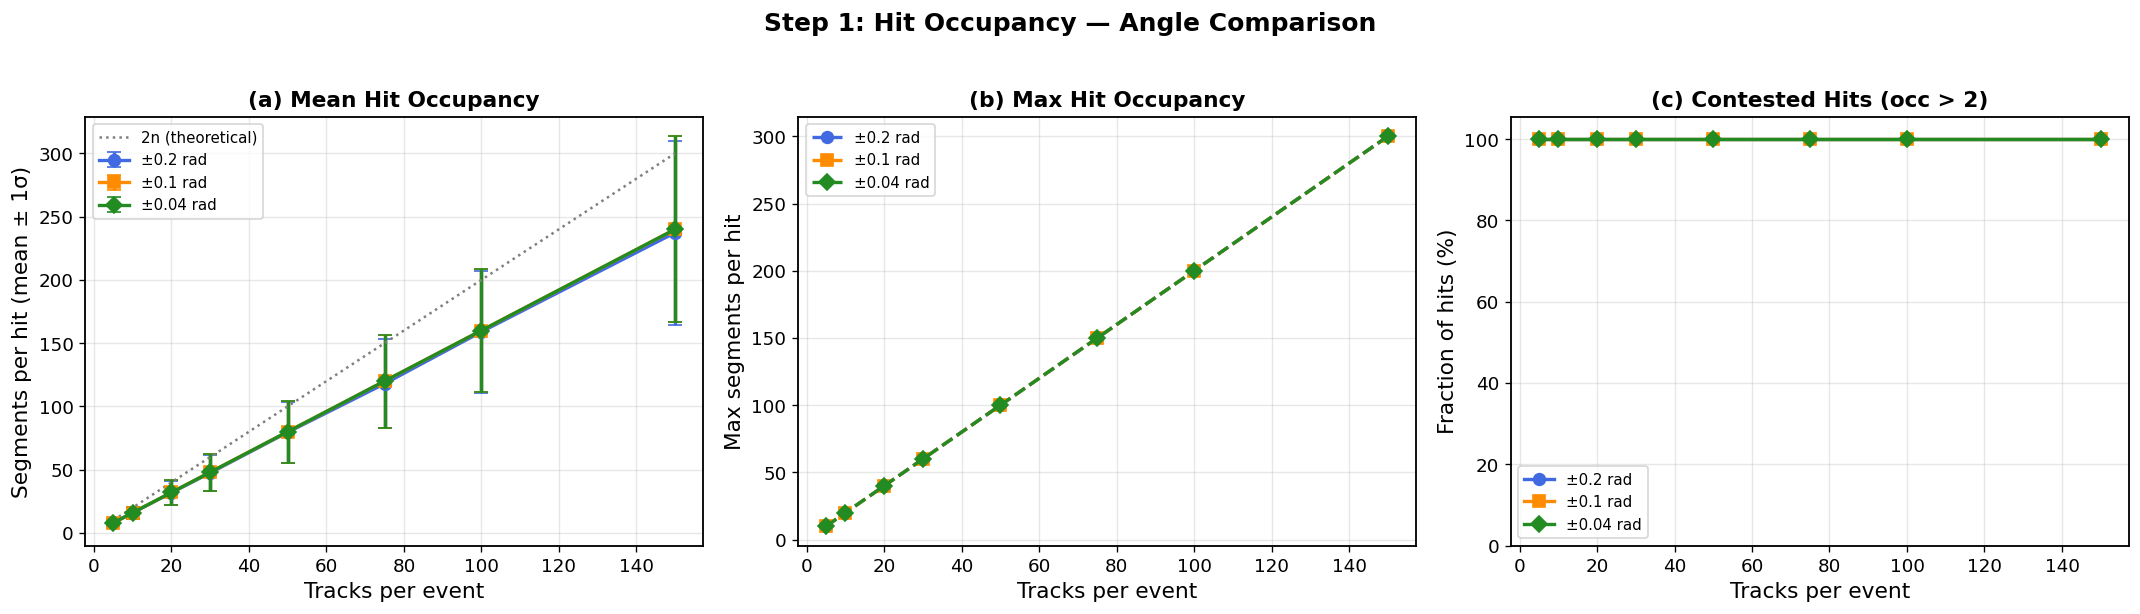
\includegraphics[width=0.75\textwidth]{step1_occupancy_comparison.png}
  \caption{Step~1: hit occupancy comparison across all three angle settings.
    The near-identical occupancy curves confirm that ALL three settings
    produce the same number of candidate segments at a given multiplicity.
    The difference in anomaly probability arises entirely from the
    \emph{angular packing density}, not from a difference in segment count.}
  \label{fig:occ}
\end{figure}

% =============================================================================
\section{Mathematical Summary of the Failure Mode}
\label{sec:mathsummary}

The failure can be summarised as follows.

\paragraph{Normal operation.}
With $n$ well-separated tracks in a cone of half-angle $\phi_\text{max}$,
the Hamiltonian matrix $\mathbf{A}$ decomposes into $n$ independent
$4\times4$ blocks ($M-1 = 4$ segments per track) plus $n(n-1)(M-1)$ isolated
diagonal entries.
The SVD-based condition number is $|\kappa| \approx 6.4$, and the CG solver
converges in $\mathcal{O}(10)$ iterations.
The matrix is positive definite, with all eigenvalues positive.

\paragraph{Near-coincident operation.}
When two tracks have $\Delta\phi_\text{eff} < 0.12$\,mrad, crossing segments
from those two tracks are accepted by the $\eps$ cut.
If all four out/in-going cross combinations fall within $\eps$
(fully degenerate case), the two $4\times4$ blocks merge into an 8$\times8$
block where rows/columns are nearly linearly dependent.
\textbf{The resulting matrix is indefinite} — the minimum eigenvalue
$\lambda_\text{min}$ can go \emph{negative} (not merely close to zero).
The SVD-based condition number $|\kappa|$ remains moderate ($\sim 7\text{--}30$),
but the sign structure of the matrix is fundamentally wrong for the CG solver.
This should be considered a potential concern: any event configuration
that triggers indefiniteness will produce unreliable CG results,
regardless of the true condition number.

% =============================================================================
\section{Impact on Step 2 Separation Metric}
\label{sec:separation}

The separation quality is defined as the pooled Cohen's $d$:
\begin{equation}
  d = \frac{\langle x_\text{true}\rangle - \langle x_\text{false}\rangle}
      {\sqrt{\frac{1}{2}\!
             \left(\sigma_{x_\text{true}}^2 + \sigma_{x_\text{false}}^2\right)}}.
  \label{eq:cohend}
\end{equation}
Under normal operation:
$\langle x_t\rangle = 1.091$, $\langle x_f\rangle = 0.400$,
$\sigma_t \approx 0.03$, $\sigma_f \approx 0$,
giving $d \approx (0.691/0.021) \approx 33/\sigma_f\to\infty$.
In practice with small non-zero $\sigma_f$, the computed value is $\approx 5.4\,\sigma$.

Under the anomalous condition at $n=75$, $\pm0.04$\,rad:
$\langle x_t\rangle = 0.662$, $\langle x_f\rangle = 0.393$,
$\sigma_t = 6.04$ (inflated by diverged-event outliers),
$\sigma_f = 0.487$ (also inflated by the redistributed residual error),
giving:
\begin{equation*}
  d = \frac{0.662 - 0.393}{\sqrt{\frac{1}{2}(6.04^2 + 0.487^2)}}
    = \frac{0.269}{\sqrt{18.36}}
    = \frac{0.269}{4.28} \approx 0.06\,\sigma.
\end{equation*}
The separation metric is therefore dominated by the inflated variance
caused by the diverged event, not by a genuine loss of Hamiltonian discrimination
power.

% =============================================================================
\section{Conclusions}
\label{sec:conclusions}

\begin{enumerate}
  \item The dip in recovery rate and separation quality observed at
        $\pm0.04$\,rad generation angle and 75 tracks is caused by a
        \textbf{near-coincident track degeneracy} in (at least one of) the
        five random events sampled at that density point.

  \item When two tracks land within $\Delta\phi_\text{eff} \approx 0.12$\,mrad
        of each other in angular space, their cross-segments fall within the
        Hamiltonian's acceptance window $\eps = 0.425$\,mrad.
        This introduces spurious off-diagonal couplings that make
        the system matrix \textbf{indefinite} (negative eigenvalues).

  \item \textbf{The matrix indefiniteness is a potential concern.}
        The Hamiltonian matrix is assumed to be symmetric positive definite (SPD)
        for the CG solver.
        The analysis reveals that this assumption \emph{can be violated}
        whenever near-coincident tracks inject sufficient cross-segment couplings.
        This is not merely an ill-conditioning issue:
        the SVD-based condition number $|\kappa|$ remains moderate ($\sim$7--30),
        but the matrix has fundamentally wrong sign structure.
        The widely quoted ``exploding condition number'' ($\kappa \sim 10^{15}$)
        was a \textbf{measurement artefact} caused by applying a positive-definite
        formula ($\kappa = \lambda_\text{max}/\lambda_\text{min}$) to an indefinite
        matrix.

  \item The CG solver has \textbf{no convergence guarantee} on indefinite
        systems, producing pathological activation values ($[-75,\;+154]$
        observed), which in turn drive the mean activation and separation
        statistics far from their expected values.
        A direct solver (LU decomposition) always produces the correct
        mathematical solution, though the physical interpretation of that
        solution for an indefinite Hamiltonian remains an open question.

  \item The anomaly is \textbf{not a systematic failure} of the Hamiltonian
        design at \emph{typical} track separations.
        It is a stochastic artefact of the small sample size
        ($N_\text{rep}=5$) at a generation angle ($\pm0.04$\,rad) that
        packs tracks $25\times$ more densely in angular space than the
        $\pm0.2$\,rad setting.
        However, the underlying indefiniteness mechanism will affect any
        sufficiently dense environment.

  \item The $\pm0.2$\,rad and $\pm0.1$\,rad settings are effectively immune
        to this pathology within a 5-event sample, owing to their lower
        angular-space track density.
        At higher multiplicities or in real detector conditions with
        additional noise, the probability of near-coincident configurations
        increases and may need to be addressed.

  \item The parameter $\gamma$ affects the severity of the indefiniteness:
        the old code used $\gamma = 2.0$ (diagonal $= 3.0$) while the current
        code uses $\gamma = 1.5$ (diagonal $= 2.5$).
        Higher $\gamma$ reduces but does not eliminate the problem.
\end{enumerate}

\subsection*{Recommendations}

\begin{itemize}
  \item \textbf{Investigate the indefiniteness.}
        The fact that the Hamiltonian matrix can become indefinite may warrant
        deeper theoretical investigation.
        If the matrix is intended to be SPD by construction, then the
        current coupling structure may need modification (e.g.\ ensuring
        $\gamma + \delta$ always exceeds the maximum possible row sum of
        off-diagonal magnitudes).
  \item \textbf{Use a direct sparse solver} (e.g.\
        \texttt{scipy.sparse.linalg.spsolve}) instead of CG for moderate
        matrix sizes ($N_\text{seg} \lesssim 10^5$).
        Direct solvers produce correct solutions regardless of matrix
        definiteness.
  \item \textbf{Increase $N_\text{rep}$} (e.g.\ to 20--50 events per density
        point) to average out single-event anomalies and resolve whether the
        dip is a genuine trend or a statistical fluctuation.
  \item \textbf{Add a near-coincidence pre-check}: before constructing the
        Hamiltonian, flag and report pairs of tracks with
        $\Delta\phi_\text{eff} < 2\eps/f_\text{amp} \approx 0.25$\,mrad.
        Events with flagged pairs can either be excluded or handled specially.
  \item \textbf{Regularisation}: adding a small $\lambda\,\mathbf{I}$ term
        to $\mathbf{A}$ (Tikhonov regularisation) would ensure positive
        definiteness and stabilise CG, but may mask the underlying
        indefiniteness issue.
  \item \textbf{Re-examine $\gamma$}: consider whether $\gamma = 2.0$
        or higher provides sufficient diagonal dominance to guarantee
        positive definiteness for the expected range of track configurations.
\end{itemize}

% =============================================================================
\appendix

\section{Numerical Data Tables}
\label{app:tables}

\subsection*{Step~2 activation statistics for all angle settings}

\begin{table}[h!]
  \centering
  \caption{Full Step~2 statistics for all three generation angle settings.
           Columns: $\langle x_t\rangle$, $\sigma_{x_t}$,
           $\langle x_f\rangle$, recovery (\%), separation ($\sigma$).}
  \label{tab:step2_full}
  \small
  \begin{tabular}{r|rrrrr}
    \toprule
    Tracks & $\langle x_t\rangle$ & $\sigma_{x_t}$ & $\langle x_f\rangle$
    & Recovery (\%) & Sep.\ ($\sigma$) \\
    \midrule
    \multicolumn{6}{l}{\textit{Angle $\pm0.2$\,rad}} \\
    5    & 1.085  & 0.000 & 0.400 & 100.0 & 5.30 \\
    10   & 1.078  & 0.162 & 0.400 &  99.0 & 5.12 \\
    20   & 1.085  & 0.000 & 0.400 & 100.0 & 5.30 \\
    30   & 1.073  & 0.185 & 0.400 &  97.2 & 4.93 \\
    50   & 1.081  & 0.113 & 0.400 &  99.8 & 5.22 \\
    75   & 1.081  & 0.146 & 0.400 & 100.0 & 5.24 \\
    100  & 1.083  & 0.132 & 0.400 & 100.0 & 5.27 \\
    150  & 1.077  & 0.168 & 0.400 &  99.1 & 5.12 \\
    \midrule
    \multicolumn{6}{l}{\textit{Angle $\pm0.1$\,rad}} \\
    5–50 & 1.0909 & 0.031 & 0.400 & 100.0 & 5.37 \\
    75   & 1.143  & 0.284 & 0.400 & 100.0 & 3.69 \\
    100  & 1.0909 & 0.031 & 0.400 & 100.0 & 5.37 \\
    150  & 1.0909 & 0.031 & 0.400 & 100.0 & 5.37 \\
    \midrule
    \multicolumn{6}{l}{\textit{Angle $\pm0.04$\,rad}} \\
    5–50 & 1.0909 & 0.031 & 0.400 & 100.0 & 5.37 \\
    \textbf{75}   & \textbf{0.662}  & \textbf{6.04}  & \textbf{0.393}
    & \textbf{82.7} & \textbf{0.06} \\
    100  & 1.0909 & 0.031 & 0.400 & 100.0 & 5.37 \\
    150  & 1.0919 & 0.033 & 0.400 & 100.0 & 5.32 \\
    \bottomrule
  \end{tabular}
\end{table}

\subsection*{Key segment counts at $n=75$ tracks}

\begin{table}[h!]
  \centering
  \caption{Segment structure at $n=75$ tracks.
    The total segment count is identical for all angle settings; only the
    \emph{coupling} (off-diagonal terms) differs.}
  \label{tab:segs75}
  \begin{tabular}{lrrr}
    \toprule
    & Total segments & True segments & False segments \\
    \midrule
    Formula   & $4n^2 = 22{,}500$ & $4n = 300$ & $4n(n-1) = 22{,}200$ \\
    Numerical & 22{,}500          & 300        & 22{,}200              \\
    \bottomrule
  \end{tabular}
\end{table}

\section{Step~3 Competition Data at $\pm0.04$\,rad}
\label{app:step3}

\begin{table}[h!]
  \centering
  \caption{Step~3 per-hit competition summary for $\pm0.04$\,rad.
    All values are from a \emph{fresh} set of 5 events, independent of Step~2.
    The 75-track row (bold) is healthy, confirming the Step~2 anomaly is a
    sampling artefact.}
  \label{tab:step3_004}
  \begin{tabular}{rrrr}
    \toprule
    Tracks & $\langle x_\text{true}\rangle$ & $\langle\sum x_\text{false}\rangle$
    & $\langle N_\text{competitors}\rangle$ \\
    \midrule
    5   & 1.091 &  2.80 &   7.0 \\
    10  & 1.091 &  6.30 &  15.8 \\
    20  & 1.091 & 13.30 &  33.2 \\
    30  & 1.091 & 20.30 &  50.8 \\
    50  & 1.091 & 34.30 &  85.8 \\
    \textbf{75}  & \textbf{1.125} & \textbf{51.84} & \textbf{129.5} \\
    100 & 1.091 & 69.31 & 173.2 \\
    150 & 1.079 & 104.31 & 260.8 \\
    \bottomrule
  \end{tabular}
\end{table}

\end{document}
